\documentclass[nofilelist]{cslthse-msc}
% to show a list of used packages at the end of the document, delete the nofilelist option
%\documentclass{cslthse-msc} 
\usepackage[utf8]{inputenc}
\usepackage[english]{babel}
\usepackage{amsmath}
%\usepackage{amsfonts}
%%\usepackage{amssymb}
\usepackage{amsthm}
%\usepackage{makeidx}
\usepackage{graphicx}
\usepackage[titletoc, header, page]{appendix}
\usepackage{transparent}
\usepackage{algpseudocode}
\usepackage{amsmath}
\usepackage{titlesec}

% used to display the used files at the end. Select nofilelist as a package option to disable this
\listfiles % initialize

%\geometry{showframe}
%better like this?
\student{Alexander Sandström}{alexander.h.sandstrom@gmail.com}
%\students{Flavius Gruian}{Flavius.Gruian@cs.lth.se}{Camilla Lekebjer}{Camilla.Lekebjer@cs.lth.se}

\thesisnumber{} % Magic Number! Do not change unless Birger Swahn asks you to do so!
% default is Master. Uncomment the following for "kandidatarbete"/Bachelor's thesis
%\thesistype{Bachelor}{Kandidatarbete}

%\title{Formatting a Master's Thesis}
\title{Drones for Sea Rescue: Lab and Field Experiments on Camera Gimbal Control}
\svensktitel{Drönare inom Sjöräddning: Labb- och Fältexperiment på Kamerastyrning}


%\onelinetitle
%\twolinestitle
\threelinestitle
%\fourlinestitle

%\subtitle{A suitable subtitle}
\company{the Swedish Sea Rescue Society and the Department of Electrical and Information Technology, Lund University}
\supervisors{Fredrik Falkman, \href{mailto:fredrik.falkman@ssrs.se}{\texttt{fredrik.falkman@ssrs.se}}}{William Tärneberg, \href{mailto:william.tarneberg@eit.lth.se}{\texttt{william.tarneberg@eit.lth.se}}}
\examiner{Maria Kihl, \href{mailto:maria.kihl@eit.lth.se}{\texttt{maria.kihl@eit.lth.se}}}

\date{\today}
%\date{January 16, 2015}

\acknowledgements{
I would first like to thank Fredrik Falkman for introducing me to the EOS project and for providing the necessary hardware resources to enable the thesis work. I am also grateful to my supervisor, William Tärneberg, along with Haorui Peng for their many ideas and technical advice. Regarding the experiment, Kjell Brunnström and his colleagues at RISE Kiste were of great help both during its development and evaluation. Lastly, I want to thank Oscar Sanner for letting me use his robot Oliver as a part of my test bed and for being a great lab partner throughout the semester.

The user experiment in this M.Sc. project has been partly supported by Sweden´s Innovation Agency (VINNOVA, dnr. 2021-02107) through the Celtic-Next project IMMINENCE (C2020/2-2), which is hereby gratefully acknowledged.
}

\theabstract{
The objective of this thesis has been to improve the camera controls of a fixed-wing drone to be used in maritime search-and-rescue operations by the Swedish Sea Rescue Society (SSRS). A gimbal control interface (GCI) has been implemented that displays the video feed of the drone camera while taking control inputs from a joystick that moves its view in real-time. 

In the thesis, the GCI has been used to conduct two experiments. The first was in a lab setting using a Quality of Experience framework, where the effects of latency on a camera operator given a specific task were studied. The results from this experiment show that higher latency worsens both the operator's ability to perform the task as well as their subjective experience with the system. Comparing the rates at which they worsen, the data suggests that task performance decreases exponentially while the subjective experience decreases linearly, although more trials are required to establish their exact relationships. 

In the second experiment, the GCI was integrated with the pre-existing systems of the SSRS and used in a test flight over the Gothenburg archipelago. During the flight, joystick control was deemed most suitable when flying in a straight line, either for surveying or following a moving object.

In conclusion, a versatile test bed allowing for manual control of a drone-mounted camera-gimbal was developed. For the SSRS, the GCI will serve as a starting point for controlling the drone's camera. Additionally, the GCI and the test bed developed in the thesis could be used in further research to better understand the relationship between different network parameters and an operator's quality of experience.
}

\keywords{Drones, Search and Rescue, Unmanned Aerial Vehicle, UAV, gimbal, camera control, ArduPilot, Quality of Experience, QoE}

%% Only used to display font sizes
\makeatletter
\newcommand\thefontsize[1]{{#1 \f@size pt\par}}
\makeatother
%%%%%%%%%%

\begin{document}

\renewcommand{\bibname}{References}

\makefrontmatter


\chapter{Introduction}
The use of unmanned aerial vehicles (UAVs) has skyrocketed during the last decades, and with consumers now having access to drones, a once mainly military technology is seeing more and more use in the civilian sector, with uses in cinematography, agriculture as well as search and rescue (SAR). The main selling point of the UAV is its' ability to provide aerial data (usually imagery) at a fraction of the cost of manned aircraft, making it a viable alternative for many expensive, remote and dangerous applications.

The use of drones and other small electric vehicles in research as well as in the DIY space has also led to the rise of several open-source software initiatives, which provide off-the-shelf software both for the on-board control of the vehicle as well as the ground control software (GCS) used for planning and monitoring missions. 

Although rotor drones are the most common consumer drones, fixed-wing drones are expected to have a lot of use cases due to their increased battery time and velocity. Despite these advantages, obtaining imagery from a fixed-wing drone remains more difficult than from a rotor drone, as the fixed-wing needs airspeed to stay in flight and will thus eventually fly past a stationary target. To solve this problem, a mechanical gimbal can be used to change the direction of the camera. The person operating the camera can also be assisted by software that can adjust the gimbal's direction based on the drone's position and orientation, either to stabilize the image or to target a specific object or GPS point.

The Swedish Sea Rescue Society (SSRS), responsible for over 90\% of sea rescues in Sweden \cite{ssrs}, is running a project with Chalmers, Infotiv, Airpelago and RISE called Eyes-on-Scene (EOS), investigating the use of drones to provide early imagery of a maritime incident to rescue personnel on their way to the scene. In the project, a fixed-wing drone carrying a gimbal-mounted camera has been developed on the open-source platform ArduPilot. A web application has also been built to ease the process of planning and monitoring missions as well as providing and recording the video feed from the drone camera.

In the project thus far, the drone has flown several waypoint missions in the archipelago of Gothenburg where the SSRS has a permit to operate drones beyond visual line-of-sight (BVLOS). The only way to control the orientation of the camera has been to upload a GPS point to the drone, also known as a "Region of Interest" (ROI), towards which the autopilot will then point the camera. Unfortunately, ROIs are susceptible to errors in all three axes, latitude, longitude and altitude, with adjustments in any of the axes usually being necessary once the ROI is uploaded. As the process of uploading an ROI is a lengthy process, the SSRS has requested a way to manually control the direction of the camera, either with a joystick or with the arrow keys. However, they suspect that with manual controls, the delay in the communication between the drone and its operator will have a greater effect on his or her experience with the system, and thus want to investigate these effects in more detail.

The rest of this chapter will provide the scope of the thesis project as well as an overview of the report structure.

\section{Scope}
\label{sec:scope}
The principal goals of the thesis work were:
\begin{description}
   \item[G1] Implement software based on the current system from the SSRS capable of manually controlling the camera-gimbal, for example with a joystick or the arrow keys. 
   \item[G2] Investigate the effects of latency on a camera operator. 
   \item[G3] Integrate the software controlling the gimbal into the existing drone system of SSRS.
   \item[G4] Evaluate the manual gimbal controls during flight and compare them to the existing ROI mode.
\end{description}

\section{Report Structure}
In the second chapter, a more elaborate background is given on UAVs, the SSRS, the EOS project as well as the research field of Quality of Experience (QoE). A technical background is also given with descriptions of the provided hardware and pre-existing software packages. In the third chapter, the implementation done in the thesis is presented. In the fourth chapter, the two experimental procedures are presented. In the fifth chapter, the results from said experiments are presented. In the sixth chapter, the results are compared to the state-of-the-art and are also evaluated on their strengths, weaknesses, limitations as well as sustainability and ethics. In the seventh chapter, the conclusions from the results are summarized. Lastly, in the eighth chapter, possible future work is presented.

\chapter{Background}
First, this chapter will give background on the particular UAV used, the SSRS and the EOS project. Then, the research field of QoE will be introduced along with the related work. Lastly, a technical background will be given to the already finished hardware and software modules.  

\section{The UAV}
\label{sec:fixed-wing-uav}
The UAV has a fixed-wing airframe and the only equipment it carries is a single camera gimbal. While it can be launched manually, the final system will use a launchpad for takeoff and land either on a rescue vessel or in the water, where it can be picked up by the rescue crew. Pictures of the UAV can be seen in Figure \ref{fig:fv-drone-pics}. 

The following subsection will introduce some basic aviation terminology. For a description of the specific components relevant to the thesis work, they are detailed in section \ref{sec:uav-components}.

\begin{figure}[htp]
   \centering
   \rotatebox{90}{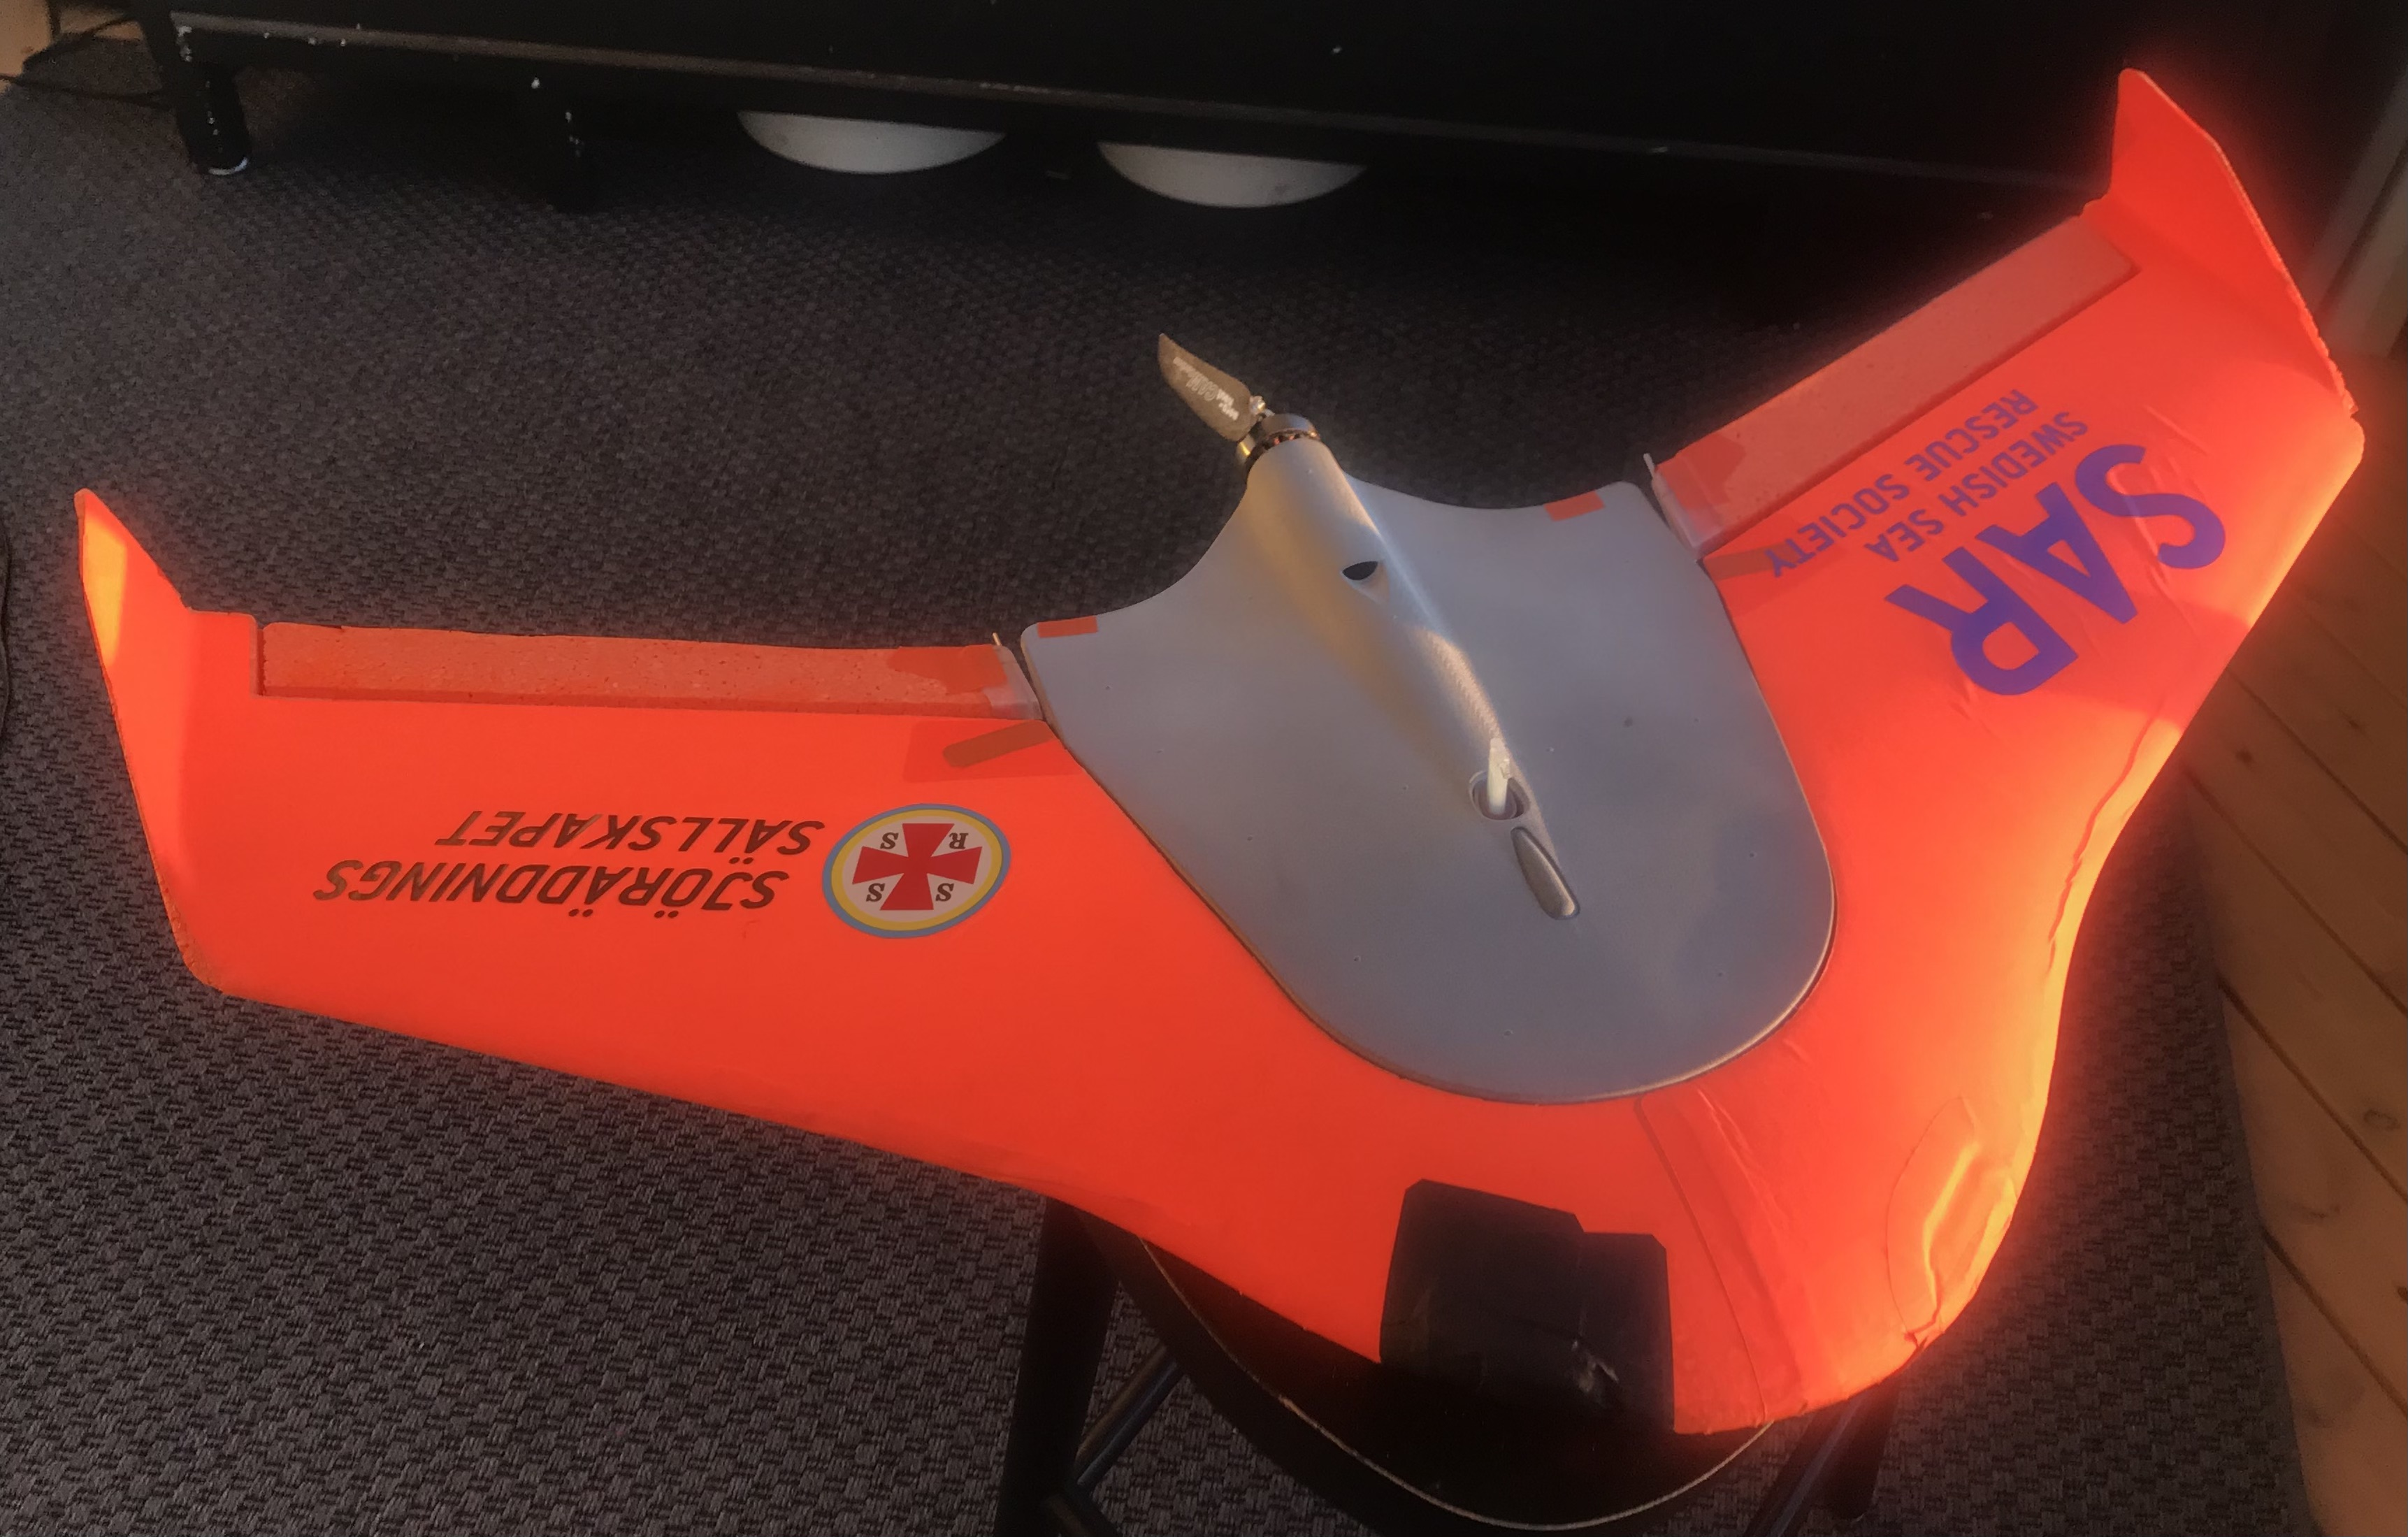
\includegraphics[width=.7\textwidth]{images/fv-3.jpg}}
   \includegraphics[width=.467\textwidth]{images/flying-drone.jpg}
   \caption{The SSRS fixed-wing drone. The left picture shows the drone from above. In the right picture, the drone is seen in flight with the gimbal and camera visible. Right picture credits: Mats Ryde.}
   \label{fig:fv-drone-pics}
\end{figure}

\subsection{Aviation Terminology}
In aviation, there are special terms for orientation used commonly when talking about the axes of the aircraft or its equipment. In Figure \ref{fig:aircraft-axes} the axes are shown for an aircraft. Roll is the rotation around the longitudinal axis, pitch is the rotation around the lateral axis and yaw is the rotation around the vertical axis. The axes are named the same when talking about the axes of the gimbal, although sometimes yaw and pitch are referred to as pan and tilt.

\begin{figure}[!hbt]
   \centering
   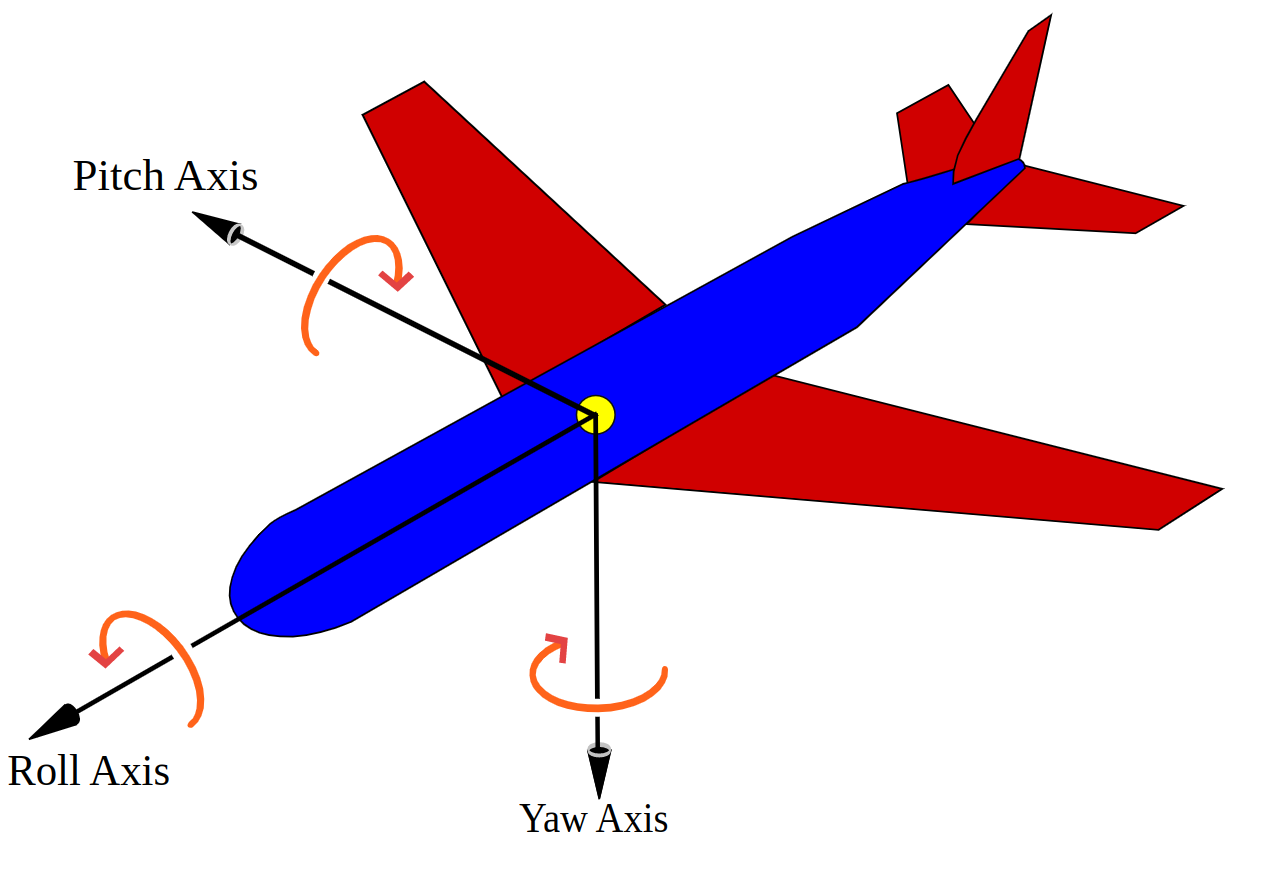
\includegraphics[scale=0.25]{images/pitch-yaw-roll.png} 
   \caption{Illustration of the roll-, pitch- and yaw-axes of an aircraft. Image credit is given to \cite{aircraft-axes-pic}.}
   \label{fig:aircraft-axes}
\end{figure}

\section{The Swedish Sea Rescue Society}
As can be read on their website \cite{ssrs}, the Swedish Sea Rescue Society (SSRS) is a non-profit organization that was founded at a conference in Stockholm in 1906 due to Sweden receiving criticism of its poor sea rescue. Today, it is a foundation with 40 employees and over 143 000 members, and with 2400 volunteers manning their 260 rescue vessels, they contribute to around 90\% of all sea rescues in Sweden all year around.

\subsection{Innovation}
As stated in their statutes \cite{ssrs-statues}, the mission of the SSRS is not solely to carry out these rescue missions, but also to innovate and collaborate in the area of maritime rescue as well as other aiding activities in society as a whole. As a result of this, the drone project that this thesis forms part of has been conceived along with other innovation projects such as foiling rescue boats and improved rescue vehicles \cite{surtsey-innovation}.

\section{Drone Project: Eyes On Scene}
The Eyes-On-Scene project is a research and innovation project initiated in 2021 by the SSRS, Chalmers, Infotiv, Smartplanes and Airpelago. It is partially funded by the Swedish Transport Administration as part of their airspace portfolio and was set out to explore the possibilities of using UAVs as a support tool for sea rescue operations. A brief description of the different roles of the stakeholders is given in the following description:

\begin{description}
   \item[The Swedish Sea Rescue Society] Provide domain knowledge and requirements for the project. 
   \item[Airpelago] Develop mission control software.
   \item[Smartplanes] Develop the drone hardware.
   \item[Chalmer's University of Technology] Evaluate the project from a human factors perspective.
   \item[Infotiv] Develop the launcher used for takeoff.
\end{description}

The current interface developed for mission control allows for flying to and loitering around (circling) waypoints given on a map where other naval and aerial traffic is also displayed in real-time. The map also shows the zones in which one is not allowed to fly, i.e. close to airports or military zones. The interface provides video from the drone camera which is recorded and accessible after the mission. In the current interface, it is possible to set an ROI by selecting a point on a map and uploading the new waypoint to the drone.

\section{Quality of Experience}
Quality of Experience is an emerging research field that is concerned with the user's experience in multimedia systems. It is an inherently multidisciplinary field that has close ties to the field of User Experience and Human-Computer Interaction. QoE is also closely related to the field of Quality of Service (QoS), where technical aspects of networked systems are compared and evaluated on quantitative measurements like latency and throughput. The focus of QoE research is instead on the effects of network parameters on the user and its interaction with the networked system.

In the field of QoE, common objects of study are the effects of latency, jitter or image quality. For example, previous QoE research has been made on the effects of latency in remote log lifting through a VR headset \cite{industry4.0} and remotely controlled excavation equipment \cite{latency-impact}.

In the white paper \cite{qoe-definition}, Brunström et al. make a working definition of Quality of Experience: 

\begin{quote}
   \textit{Quality of Experience (QoE) is the degree of delight or annoyance of the user of an application or service. It results from the fulfillment of his or her expectations with respect to the utility and / or enjoyment of the application or service in the light of the user’s personality and current state.} 
\end{quote}

\section{Previous Work}

W. Tärneberg et al. \cite{industry4.0} present a QoE study with industrial equipment on an excavation site where experienced operators controlled their usual equipment remotely with different latencies introduced. They conclude that studying QoE aspects of a system is highly complex and task-dependent. They also state that the operator's experience is time-variant and can be highly dependent on external factors such as lighting conditions or network quality.

K. Brunnström et al. \cite{latency-impact} performed a study on log lifting using a head-mounted display system. In the study, latency is introduced both in the display's response to movement as well as the controls. The display delay was found to have a strong effect on nausea, but an observable effect on controller latency could only be found at latencies above 800 ms. 

As part of the Eyes-On-Scene-project, a study was performed at Chalmers by Grote et al. \cite{eos-maritime} where two maritime emergency calls were performed, one with and one without images from a UAV at the emergency site. The study showed that imagery from the accident gave the rescue personnel a sense of control before arriving at the scene, knowing what they were going to face. The crew was also faster at locating a person or object when having aerial footage of the scene.

In \cite{targetting}, M. Quigley et al. presents a test bed with a fixed-wing UAV on which they evaluate different means of gimbal control. They find that altitude estimation causes problems with ROI control, which results in the gimbal pointing at a circle around the point instead of directly at it. To address this they introduce controls for changing the altitude as well as the coordinates of the point, and they also have a mode in which the plane updates its loiter point to where the gimbal is looking. Manual controls of the gimbal are also implemented using a game controller. In their test bed, they map the left joystick to the attitude control of the aircraft while the right joystick is mapped to different states of the gimbal, instead of relative position.

\section{Pre-existing Hardware}
In this section, the hardware used in the experiments is presented.

\subsection{Drone Components}
\label{sec:uav-components}
The drone components relevant to this thesis are detailed in the following description. A picture of the internals of the drone is shown in \ref{fig:drone-internals}.

\begin{figure}[!hbt]
   \centering
   \rotatebox{90}{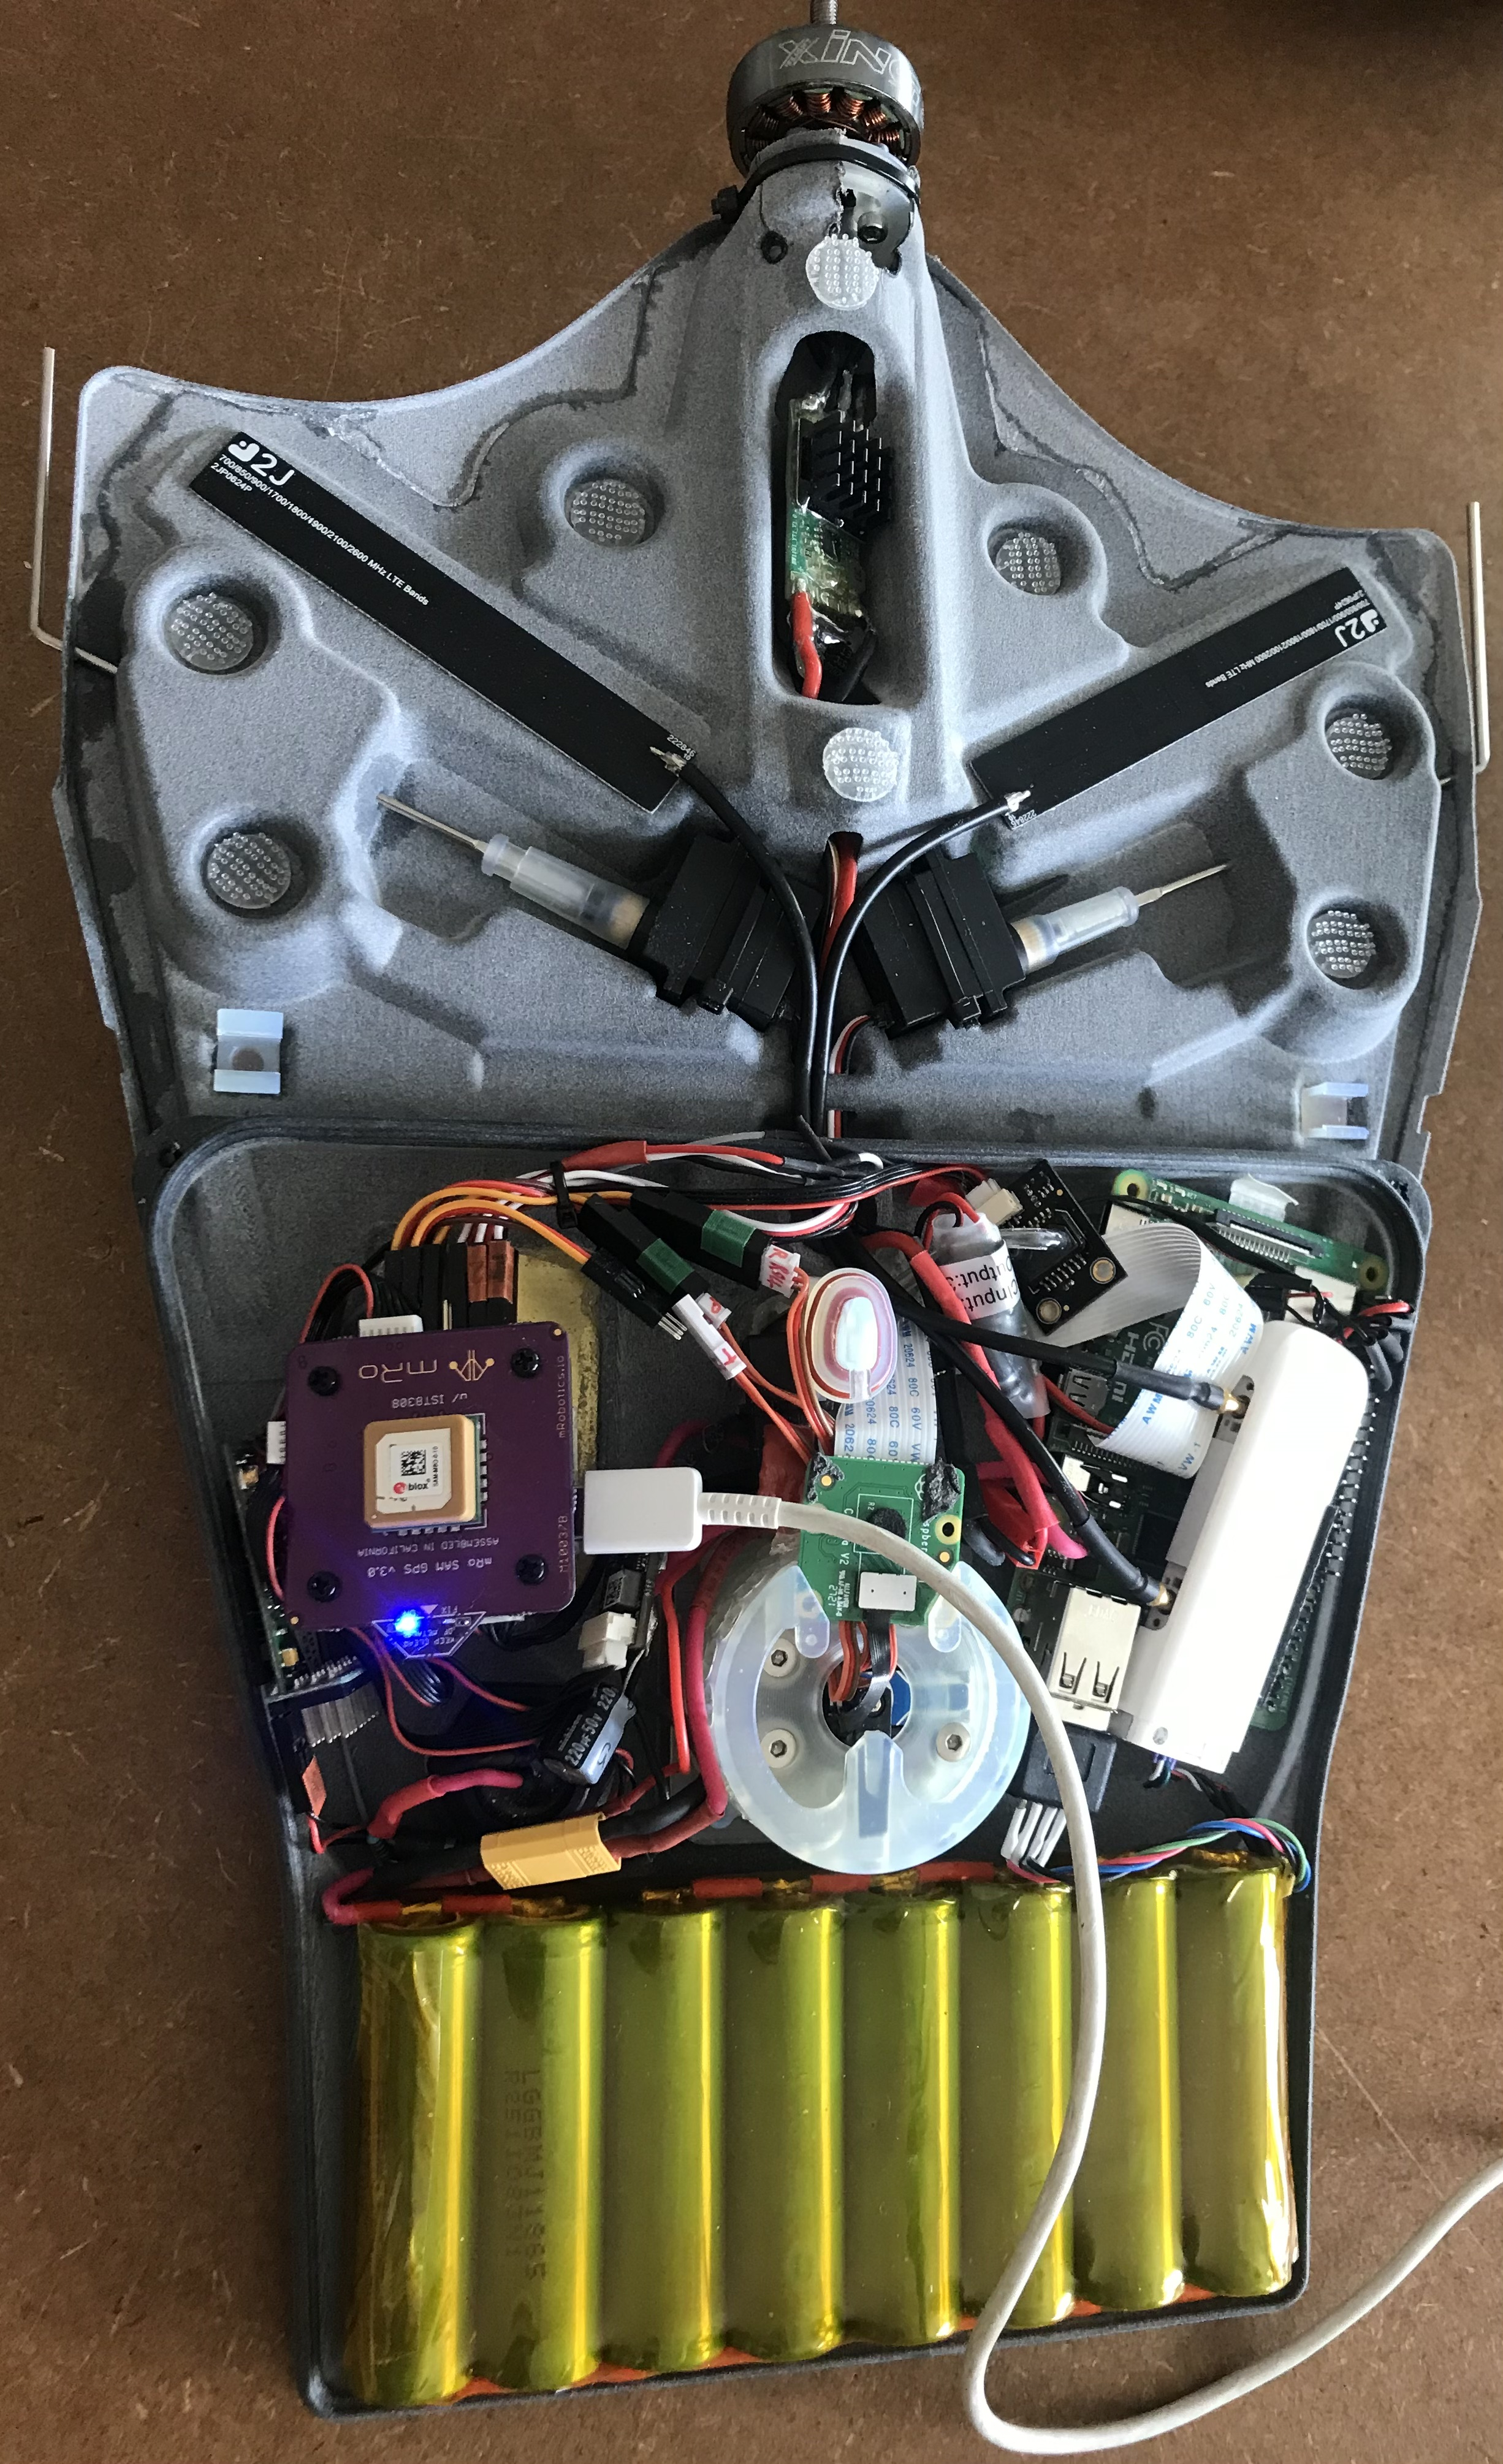
\includegraphics[scale=0.1]{images/fv-1.jpg}} 
   \caption{The housing of the drone's components. On the left side, the motor, antennas and control surface servos are visible. In the housing to the right, from top to bottom: RPi with a 4G modem on top, gimbal, GPS module and flight controller mounted beneath it. To the right, the battery pack can be seen.}
   \label{fig:drone-internals}
\end{figure}

\begin{description}
   \item[Pixracer R15] The Pixracer is the flight controller, which is the brain of the aircraft. It houses the chip running the ArduPlane software as well as components and connectors relevant to in-flight operations.

   \item[Raspberry Pi 4] The Raspberry Pi serves as the onboard computer, commonly known as the "companion computer" (CC) in the context of drone hardware. It is connected to the flight controller via USB and makes it possible to relay messages sent over Ethernet instead of radio, allowing the flight controller to connect to a ground station over the Internet. 
   
   \item[4G Modem] Sim-card modem giving access to the mobile network. 
   
   \item[Raspberry Pi Camera Module v2] The camera module is a small camera that is mounted on a flat surface inside the gimbal. The camera connects to the module board on top of the gimbal, which is in turn connected to the Raspberry Pi with a ribbon cable. It is capable of recording 1440x1080 video at 30 fps and has a 4:3 aspect ratio. 

   \item[Camera Gimbal] The camera gimbal on the drone is designed and manufactured by Fredrik Falkman at the SSRS. It is a 3D-printed design that has three degrees of freedom made possible by three servos connected to drive belts that control each axis of the camera. The servos are connected to the flight controller which also provides them with power. The gimbal is designed to house a small camera that when mounted looks out from the bottom of the drone. In \ref{fig:gimbal-pics} the schematics of the gimbal can be seen. 
   
   \begin{figure}[htp]
      \centering
      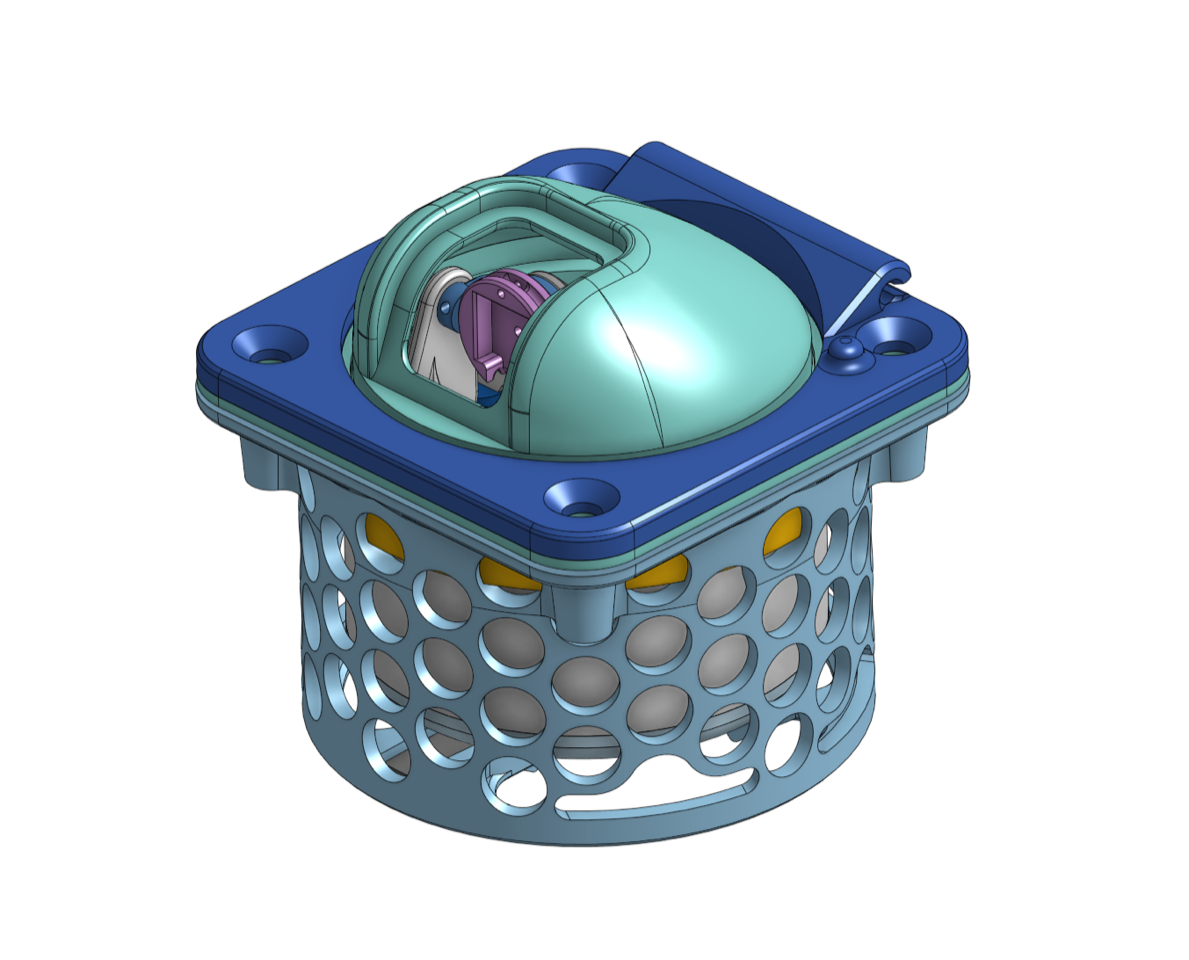
\includegraphics[width=.3\textwidth]{images/gimbal-1.png}\hfill
      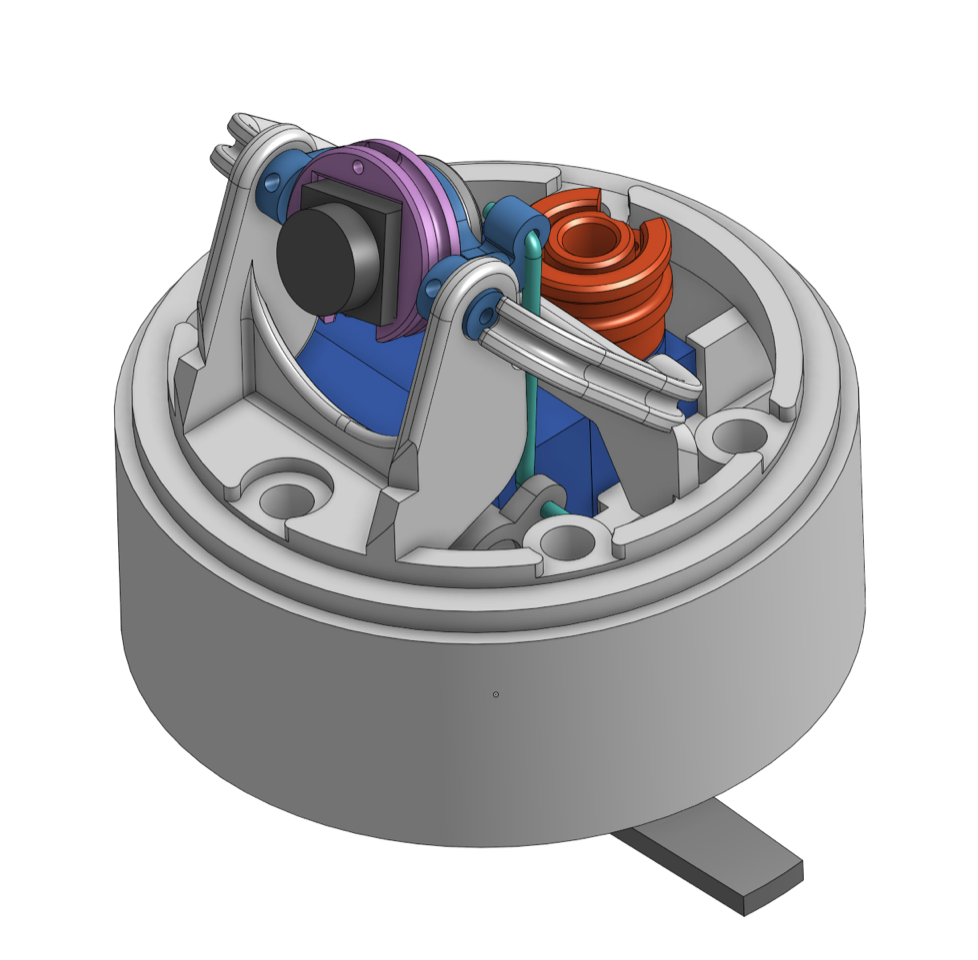
\includegraphics[width=.35\textwidth]{images/gimbal-3.png}\hfill
      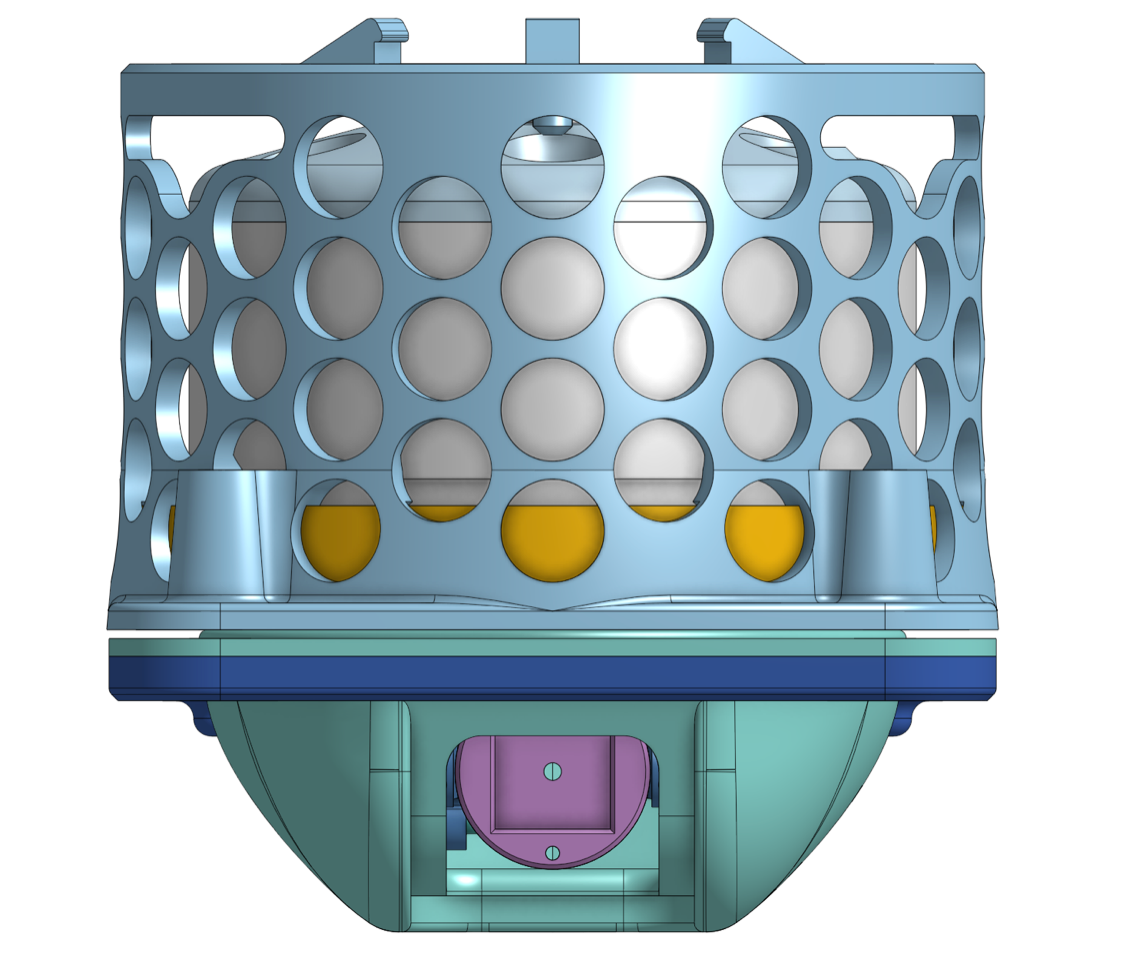
\includegraphics[width=.25\textwidth]{images/gimbal-2.png}
      \caption{Schematics of the drone gimbal. The left and right picture shows the gimbal with its full housing. In the middle picture, the housing has been removed and a mockup camera module has been inserted on the mounting plate. Beneath the camera, the three servos can be seen in blue.}
      \label{fig:gimbal-pics}
   \end{figure}
\end{description}
   
\subsection{Hoverboard Robot}
In order to introduce movement in the QoE experiment, a modified hoverboard was used. The hoverboard had two additional wheels in order to be stable and could be controlled via joystick inputs or coordinates. Its maneuvering was assisted by real-time lidar mapping of the room. The hoverboard can be seen in \ref{fig:hoverboard}

\begin{figure}[!hbt]
   \centering
   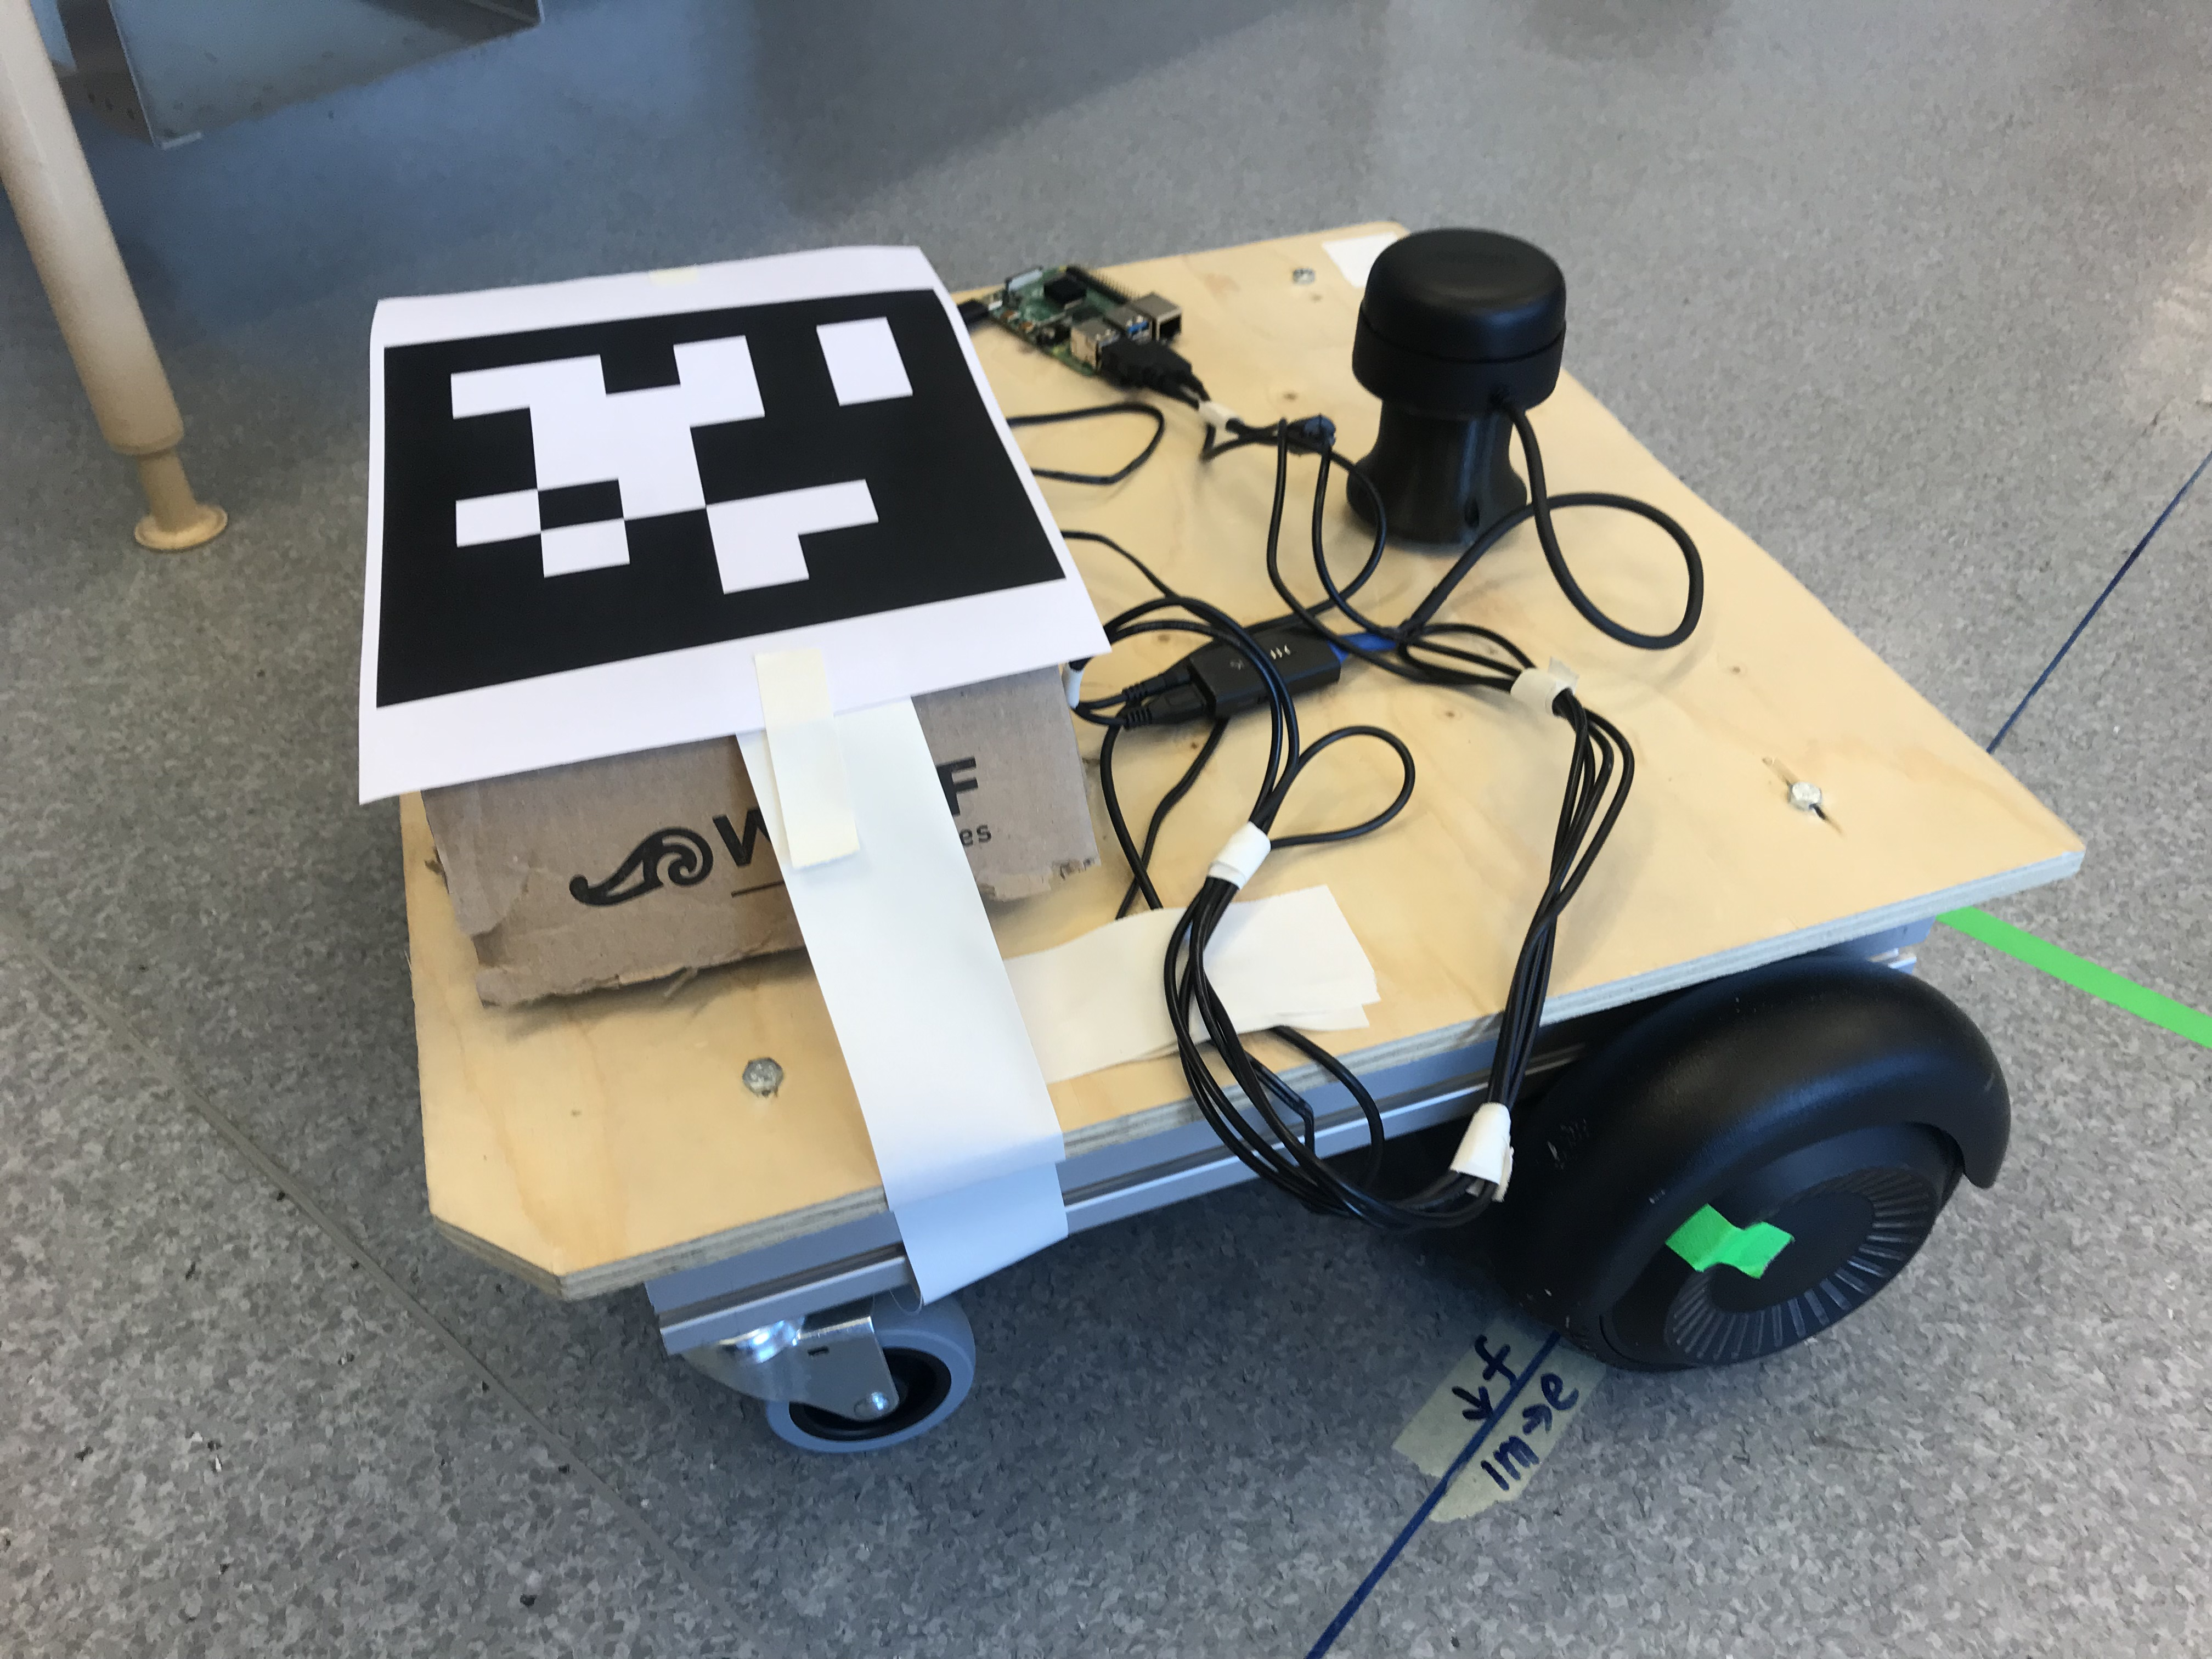
\includegraphics[scale=0.07]{images/hoverboard.jpg} 
   \caption{The hoverboard used in the test bed.}
   \label{fig:hoverboard}
\end{figure}

The average velocity of the hoverboard was determined at 0.184 m/s with a standard deviation of 0.0062 m/s. The error after each lap is presented in table \ref{tab:hoverboard-error}, and was non-accumulative over multiple laps. 

\begin{table}[!hbt]
   \centering
   \begin{tabular}{|c|c|c|c|}
      \hline
      \textbf{Axis} & \textbf{Average (mm)} & \textbf{Min (mm)} & \textbf{Max(mm)} \\
      \hline
      $x$ & $6.8 $ & $-40.2$ & $51$ \\
      \hline
      $y$ & $42.78$ & $34.9$ & $50.9$ \\
      \hline
   \end{tabular}
   \caption{Error from the origin when told to start and stop at the same position.}
   \label{tab:hoverboard-error}
\end{table}

\subsection{Apriltag}
An Apriltag is a type of low-resolution QR code often used in robotics to estimate the position and orientation of objects with the help of computer vision. It was fastened on top of the hoverboard as high as possible without blocking the lidar. The Apriltag can be seen mounted on the hoverboard in Figure \ref{fig:hoverboard}.

\section{Pre-existing Software}
In this section, the pre-existing software used in the experiments will be detailed.

\begin{description}
   \item[Firmware: ArduPlane]
   The firmware running on the flight controller is called ArduPlane, which is part of the open-source autopilot software suite ArduPilot that enables the creation of unmanned, autonomous vehicles \cite{ardupilot-org}. This software is responsible for the in-flight systems of the aircraft such as navigation and control. It is also through this software that the gimbal on the drone is controlled. It is developed by a community of developers and is available on GitHub \cite{ardupilot-github}.
   
   \item[Protocol: MAVLink]
   As can be read on their website \cite{mavlink}, MAVLink is a lightweight protocol suited for communication with drones and between drone components. It has a byte overhead of 14 bytes and allows for concurrent communication between up to 255 systems. 

   \item [Software: MAVProxy]
   MAVProxy \cite{mavproxy} is a program running on the CC whose task is to relay MAVLink messages from an ethernet interface to the flight controller's serial interface.

   \item[UV4L]
   UV4L is a video streaming service that supports several real-time communication protocols and video encodings \cite{uv4l}. Its function in the test bed is to stream the video from the camera to the web. As for video encoding, MJPEG was used.
   
   % \item[Janus Server]
   % As described on their webpage \cite{janus}, Janus is a plugin-based software that helps establish WebRTC connections. In this thesis it is used to establish the connection between the UV4L server and the web browser, enabling the peer-to-peer connection between the two devices.

   \item[Hoverboard software] The hoverboard has software that allows it to be controlled by a game controller or follow a set of points. To locate itself it uses a SLAM algorithm along with a lidar. This makes it possible to have the hoverboard run in a programmed route with little error. 
\end{description}

\chapter{Implementation}
In this chapter the hardware and software developed specifically for the thesis are detailed.

\section{Gimbal Box}
As the entire drone was not needed to test the software, a Raspberry Pi, flight controller and gimbal were mounted inside a 2L Ikea SmartStore box. The computer boards were mounted with velcro tape and the gimbal was mounted in a cutout in the bottom of the box. Pictures of the box can be seen in Figure \ref{fig:drone-setup}.

\begin{figure}[htp]
   \centering
   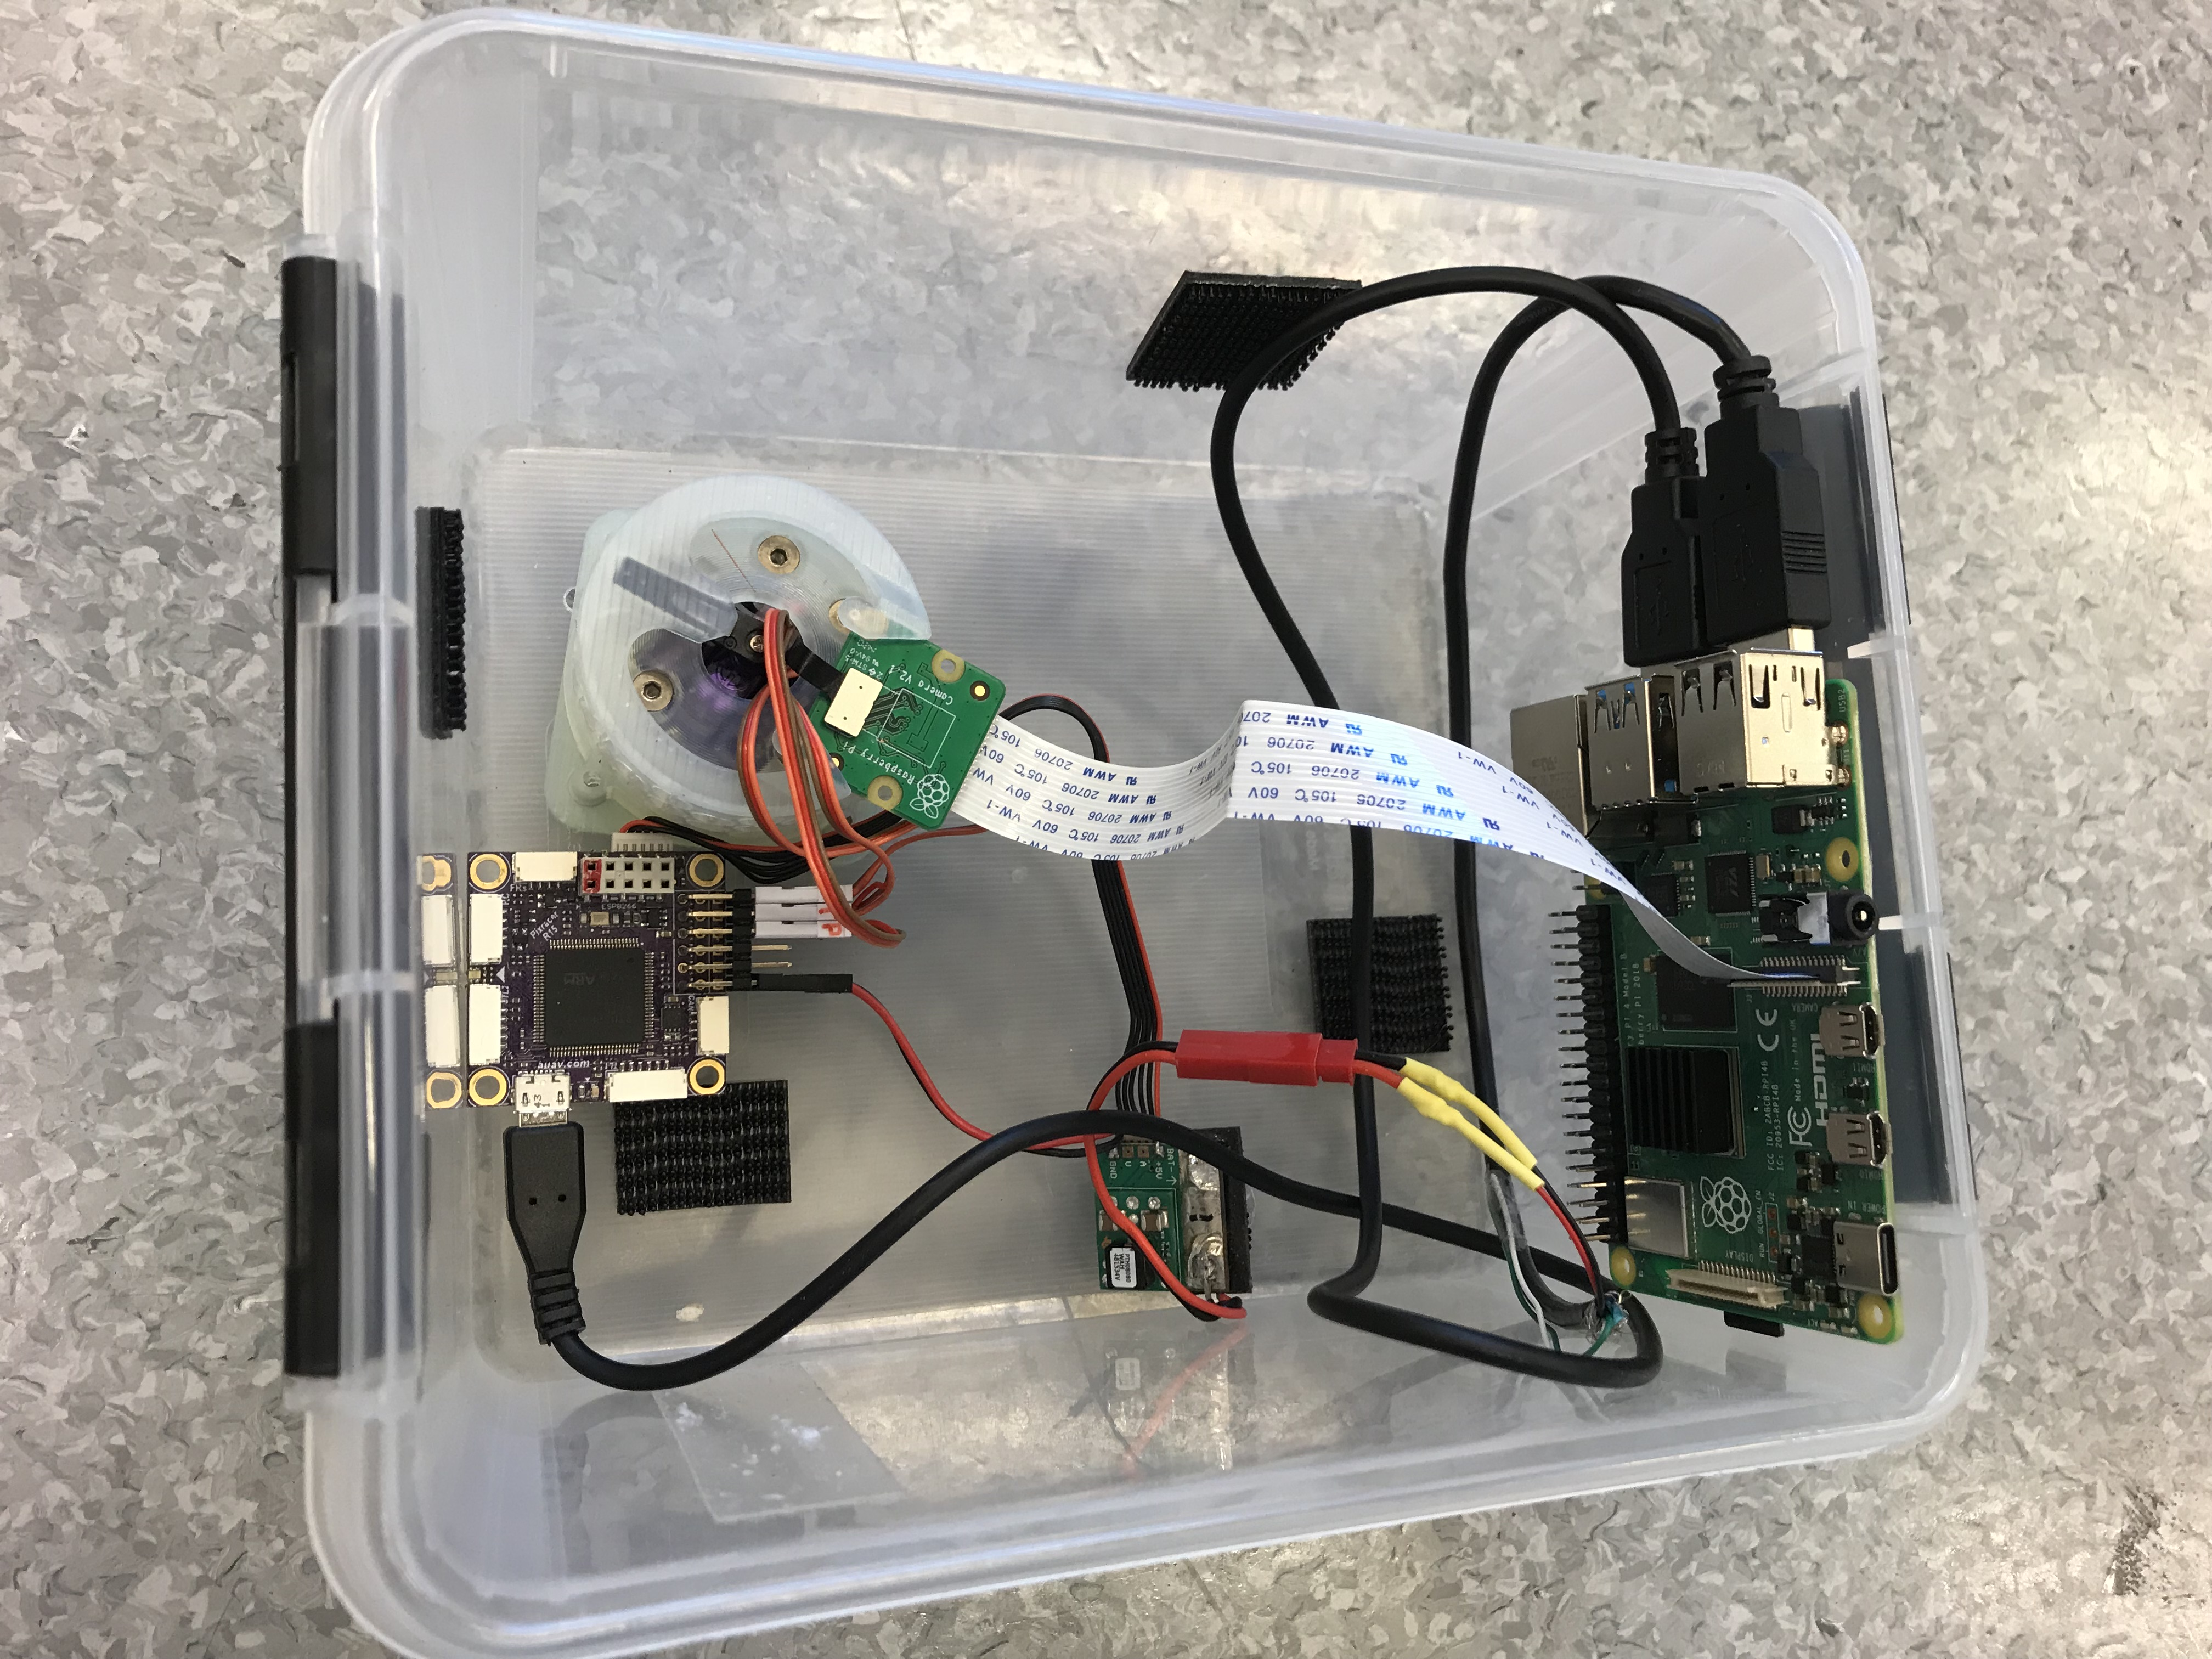
\includegraphics[width=.47\textwidth]{images/drone-box-1.jpg}\hfill
   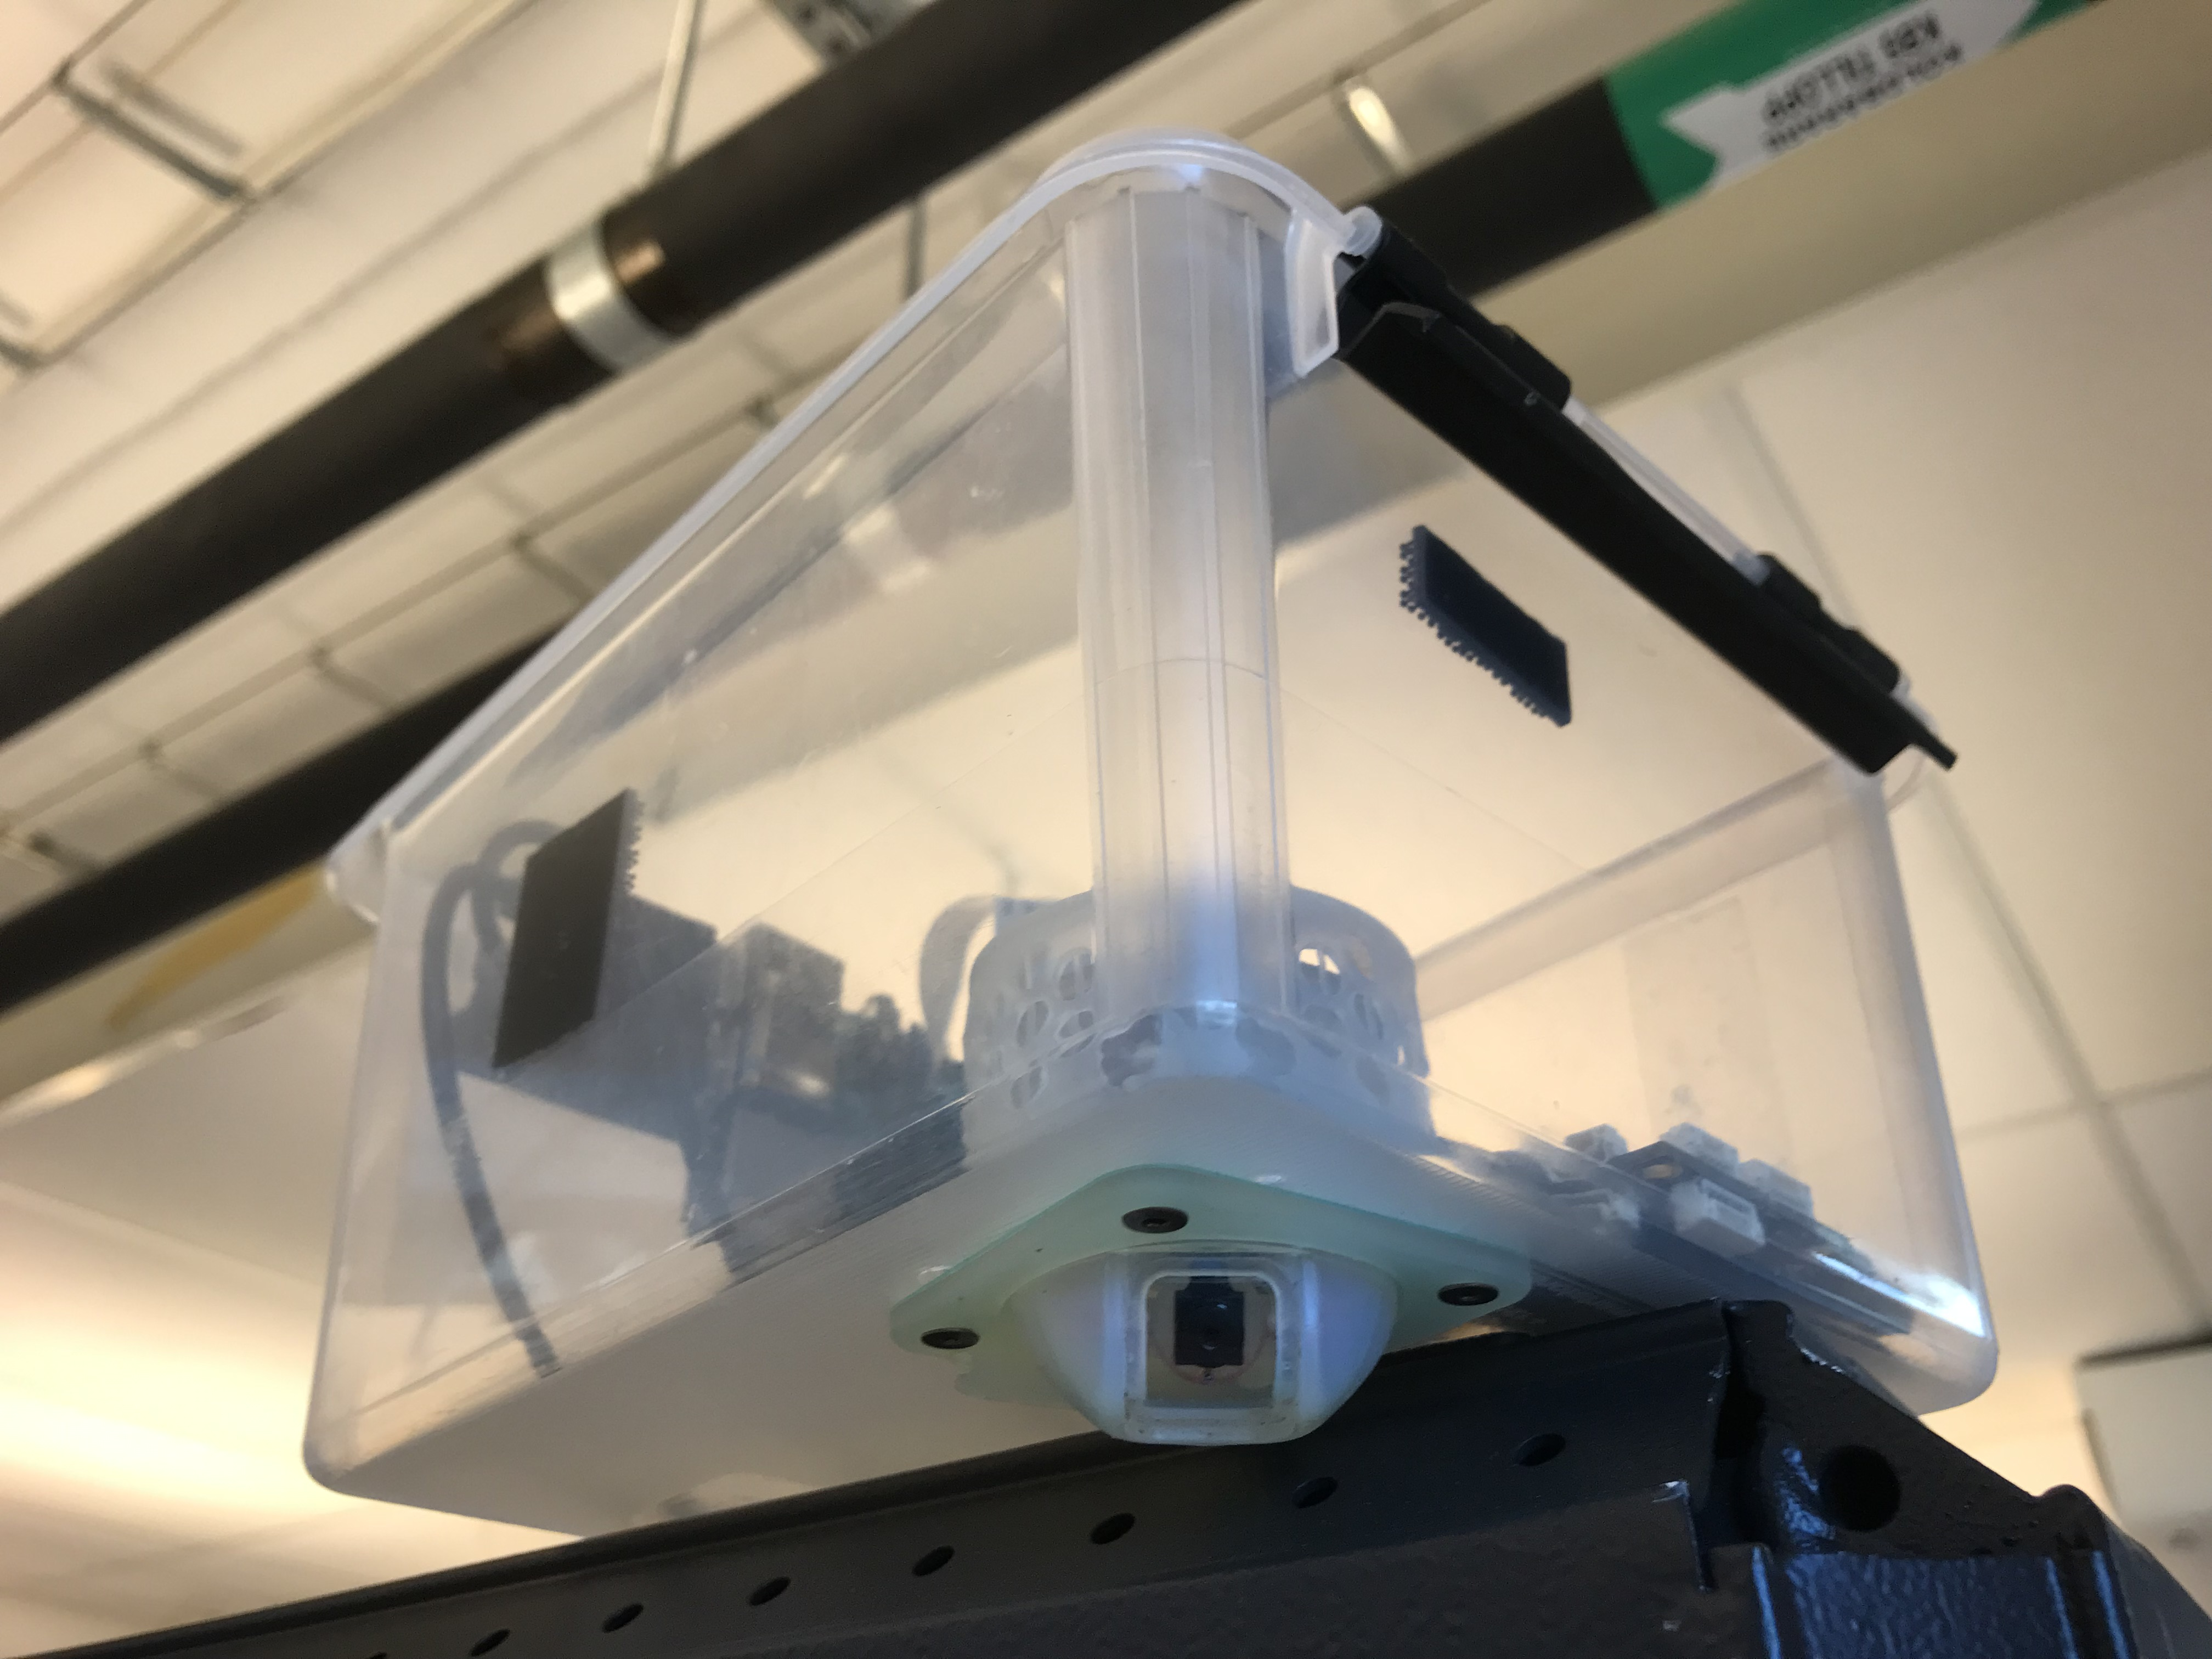
\includegraphics[width=.47\textwidth]{images/drone-box-2.jpg}
   \caption{Pictures of the box that houses the drone hardware for the experiment. The left picture shows the box from above, from the left the following components are visible: a flight controller, a gimbal with a camera module, a power supply module and a Raspberry Pi. The right image shows the box from below.}
   \label{fig:drone-setup}
\end{figure}


\section{Gimbal Control Interface}
Addressing goal \textbf{G1} of the thesis, a program was implemented in Python to display the video feed from the drone camera while taking control inputs from the operator. The inputs came from the right joystick of a PlayStation controller while the program sent messages updating the gimbal's position with a set frequency. The program could also record the video feed. A visual overview of the system is shown in Figure \ref{fig:system-overview}.
\begin{figure}[!hbt]
   \centering
   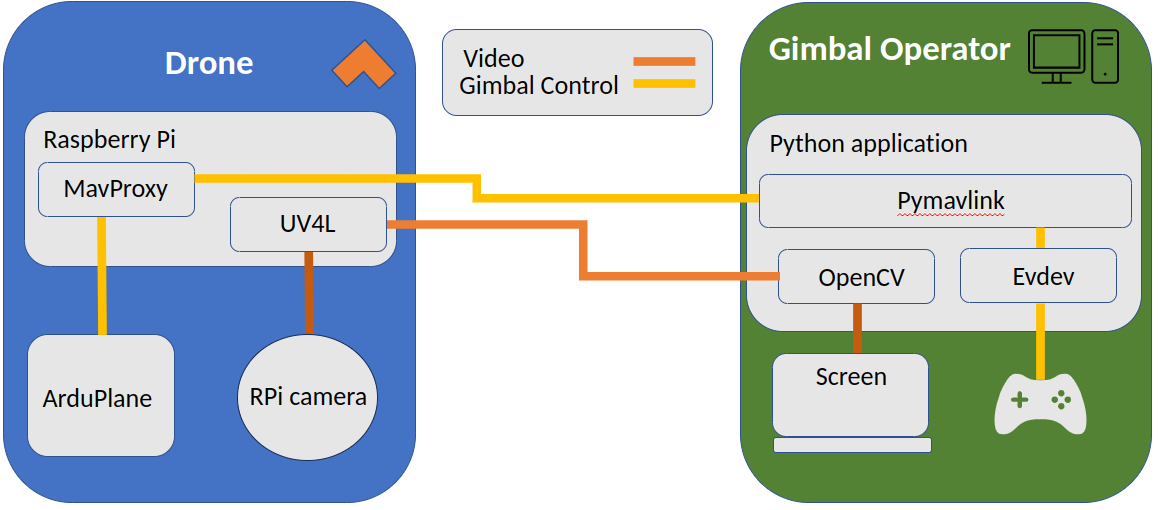
\includegraphics[scale=0.4]{images/system-overview.png} 
   \caption{An overview of the GCI with the color of the connecting lines representing which software speaks to which data they transfer. On the left, the drone and its' hardware and software components: the RPi running MavProxy and UV4L, the flight controller running ArduPlane and lastly the RPi camera module. On the right, the gimbal interface and its software components: OpenCV for obtaining and displaying video, Evdev for the controller inputs and Pymavlink for establishing the connection with the drone. }
   \label{fig:system-overview}
\end{figure}

The application was run with Python version 3.9.16 and used the following libraries:
\begin{description} 
   \item [pymavlink (v. 2.4.37)]
   An interface to communicate with MAVLink devices, available at \cite{pymavlink}. With the library, a port can be set to send and receive MAVLink messages over an IP or serial link. The system used UDP as its transport protocol but could be modified to TCP as well.
 
   \item [Evdev (v. 1.6.1)]
   A Python library for interrupt-driven input devices. It is used for reading input from the Playstation-controller. Available at \cite{evdev}.

   \item [OpenCV (v. 4.7)] 
   Open Computer Vision is a very popular library for video and computer vision tasks. It is used for displaying and recording the video feed in the gimbal interface. Available at \cite{opencv}.

   \item[Multiprocessing]
   This standard module was used to run the video tasks in different processes to not interfere with the control. The video frames were accessed and displayed by one process and then fed to another process saving each frame. For more information on the library see \cite{multiprocessing}.  
\end{description}

\subsection{Joystick Inputs}
To capture the joystick inputs, a callback function using Evdev and Python's async functionality was implemented that was called each time the controller sent an interrupt. The joystick produced an interrupt every time it moved, providing two values in the range [0, 255] (127 in the middle position). With each callback caused by the joystick, its values in both axes were scaled to the range [-127, 127] and multiplied by a sensitivity factor before being added to the pitch and yaw attributes that the class held. 

As the joystick did not produce any interrupts when standing still, even when in a non-zero position, the last joystick value had to be stored and used to update the values. This was done at a rate of 20Hz, triggered by the polling from the sending thread.

\subsection{Updating the Gimbal's Position}
When started, the GCI turned the gimbal straight ahead to synchronize the GCI's gimbal angles with the ones on the actual drone. The values for pitch and yaw were held in the previously mentioned controller thread, which was polled at a rate of 20Hz by the sending thread. If the values had changed since the last poll the sending thread would send the new pitch and yaw angles to the drone.

To maximize throughput, the protocol for communicating between the drone and the GCI was chosen to be UDP. After each message, the drone would send an acknowledgment which a system could wait for. This could be toggled in the GCI but was turned off as it did not allow a new position to be sent until the last acknowledgment had been received, introducing further latency.

\subsection{Delay}
Delays in the controls could be introduced by providing an argument to the program when started. The delay was simulated by putting each outgoing message in a queue along with a timestamp, with the program waiting until $ \text{timestamp} + \text{delay} $ was reached before sending the command. The following algorithm was used to schedule the sending of commands according to the delay: 
\begin{algorithmic}
   \While{running}
   \State $timestamp, pitch, yaw = queue.get()$ // blocking call
   \State $t_{0} = time.now$
   \State $diff = timestamp + delay - t_{0}$
   \If{diff > 0}
      \State $time.sleep(diff)$
   \EndIf
   \State $drone\_connection.send\_pitch\_yaw(pitch, yaw)$
   \EndWhile
\end{algorithmic}

\subsection{Existing Sources of Delay}
To get a rough measurement of the delay of the system, the screen and the controller were filmed on a phone at 120 FPS to measure the time between a control input to the video feed updating. This was done when connected by an ethernet cable, with network latencies <1 ms

The delay of the video feed alone was between 100-150ms while the full controller to video feedback delay was around 400ms. 

Although the sources of the delay could not be examined in any great depth some probable causes were:
\begin{description}
   \item[Message frequency] 
   While the internal model of the gimbal's orientation was updated by interrupts, the message rate to the flight controller was set to a maximum of 20Hz, resulting in a delay between 0-50ms for control update.
   
   \item [Video encoding and decoding]
   Some delay is expected to come from encoding and decoding the video. This is especially relevant with the encoding running on the resource-constrained RPi.  

   \item[MAVProxy relaying] Each message must be taken from the ethernet interface of the Raspberry Pi and be sent on the serial interface to the flight controller. An estimate of this time was not made.
   
   \item[Flight Controller] The flight controller must process the message and send the appropriate PWM signals to the gimbal servos. The processor running the firmware is a small chip and gimbal control might not be a high-priority message in the software. An estimate of this time was not made.
\end{description}

\subsection{Design Choices} 
This section aims to explain some of the design choices that were taken during the development of the gimbal interface. It can be skipped if the reader is not interested in the development process.

\subsubsection{Video streaming}
In the real drone system, the video feed is done with WebRTC. This is a modern peer-to-peer video protocol well suited for live-streaming video. The intention was to use this in the test bed as it had a low latency and was accessible through the browser. The main goal was to get the raw video feed to OpenCV to adjust image parameters as well as to be able to do detection and recording of the frames. Unfortunately, the raw video feed proved difficult to access as other video-processing software had to be used along with the peer-to-peer negotiation. In the end, the MJPEG format was chosen, as it had an acceptable delay and could be integrated only by providing an HTTP source to the OpenCV video capture module.

\subsubsection{Native vs. web}
The application that the SSRS currently uses for mission control is hosted on the web, and as such the test bed was initially developed as a web application. This proved difficult for the developer as they had limited experience working with web applications. As the number of tasks for the program to perform grew, a decision was made to implement the test bed as a native Python application instead. This made it easier to orchestrate the video and control tasks using regular UNIX processes from the Python multiprocessing library. 

With this decision, the possibility to remotely host the application was lost, but as the goal was to develop a working test bed this was deemed acceptable. 

\section{Result Script}
\label{sec:resultscript}
To extract the results from the recorded video, a Python script running a detection algorithm was implemented. The script used the following Python libraries:
\begin{description}
   \item[OpenCV] Video tasks and image processing.
   \item[dt-apriltags] Detection algorithm.
   \item[math] Mathematical operations, such as calculating the distance between two points.
   \item[sys] Iterating over directories, reading and writing files.  
\end{description}

The script took each frame of a video and ran the Apriltag detection algorithm on it. If an Apriltag was detected in the image, the distance between the center of the Apriltag and the center of the screen was saved with the corresponding frame number in a CSV file. In case of no detection, a NaN value was inserted for that frame. The video with the detection overlay was also saved for later inspection.

\begin{equation}
   \label{eq:distance}
   \overrightarrow{px} = \sqrt{(x_{hoverboard} - x_{center})^2 + (y_{hoverboard} - y_{center})^2}
\end{equation}

Pythagoras' theorem was used for calculating the pixel distance between the two points and is shown in equation \ref{eq:distance}. A frame from the detection script can be seen in Figure \ref{fig:resultcalc}.

\begin{figure}[!hbt]
   \centering
   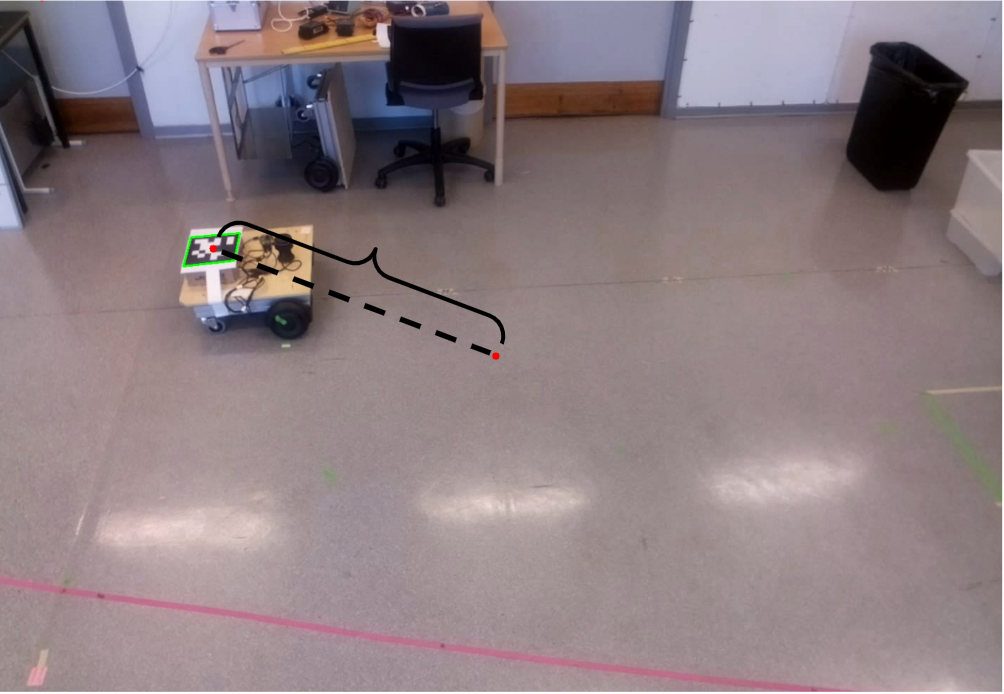
\includegraphics[scale=0.3]{images/resultcalc.png} 
   \caption{Example of a result from the detection algorithm. The green square outlines the result of the detected object and the red dot its' center. The error is the distance between the two dots as outlined by the black indicators.}
   \label{fig:resultcalc}
\end{figure}

\section{Auto-follow mode}
As a proof of concept, an auto-follow mode was developed which allowed the gimbal to follow the Apriltag. This was made using the object detection algorithm from the result script coupled with a PI controller which had the center of the image center as a reference value. Due to time limitations, this was not investigated any further.

\chapter{Experiments}
This chapter will describe the setup, procedure and evaluation of the two experiments that were performed.

\section{QoE Lab Experiment}
The goal of this experiment was to investigate the effects of latency on a camera operator, addressing goal \textbf{G2} of the thesis scope.

\subsection{Experiment Design}
The desire was to use the drone box to create a task that would be similar to what an operator would perform in a sea rescue scenario. A likely scenario was considered to be that of a drone loitering around a point while looking at the loiters center. 

With the video being the main feedback to the operator, pixel distance in an image was deemed to be a good metric for task performance. To evaluate the performance of an operator, automatic detection using an Apriltag was considered from the implementation stages of the thesis. With this approach, the number of frames that could be analyzed could be dramatically increased compared to manual evaluation.

Initial tests were done with the gimbal box sitting on top of the hoverboard while the hoverboard was moving in a circle. This would result in an upside-down loiter with the gimbal looking up at a point in the ceiling that was in the center of its loiter. The scenario is shown in Figure \ref{fig:testbed-idea-1}. After some initial testing, this was deemed to introduce several points of failure in the test bed:

\begin{figure}[htp]
   \centering
   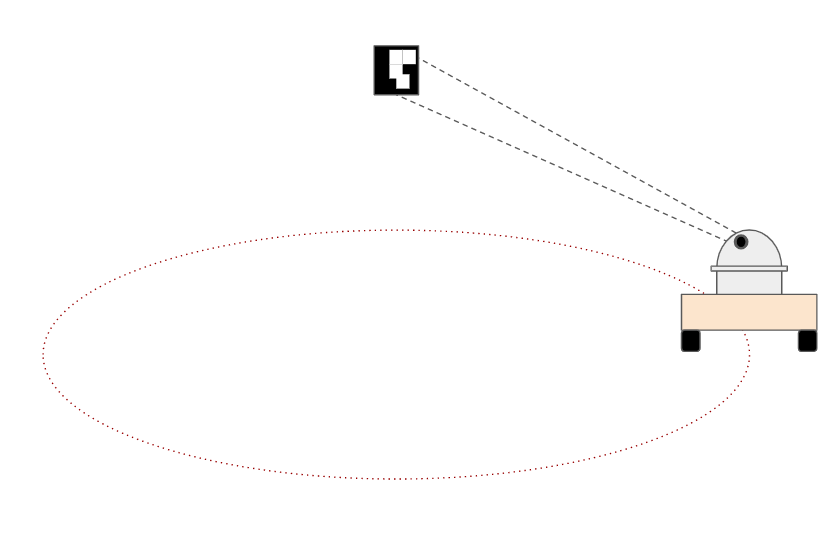
\includegraphics[width=.6\textwidth]{images/testbed1.png}
   \caption{The initial idea of the experiment setup where the camera is looking up on the Apriltag. }
   \label{fig:testbed-idea-1}
\end{figure}

\begin{enumerate}
   \item Power had to be supplied via a power bank.
   \item Network connection had to go over WiFi with substantially more delay and jitter than an ethernet cable connection. 
   \item Using automatic detection, the lighting from the ceiling and windows reduced the contrast of the Apriltag, making it harder to detect for the algorithm.
   \item When mounted, the gimbal box was higher than the lidar mounted on the hoverboard, confusing the location algorithm on the hoverboard.
\end{enumerate}

In the end, the loitering scenario was flipped, placing the gimbal box on top of a shelf and looking down at the moving robot, shown in Figure \ref{fig:testbed-idea-2}. Since the gimbal could not turn around completely, the box had to be placed next to the path where the hoverboard was running. A slit of green tape was placed on the floor in the room from which the hoverboard could run in a path 2x1m ellipse. Its path in the lab can be seen in Figure \ref{fig:exp-setup}.

\begin{figure}[htp]
   \centering
   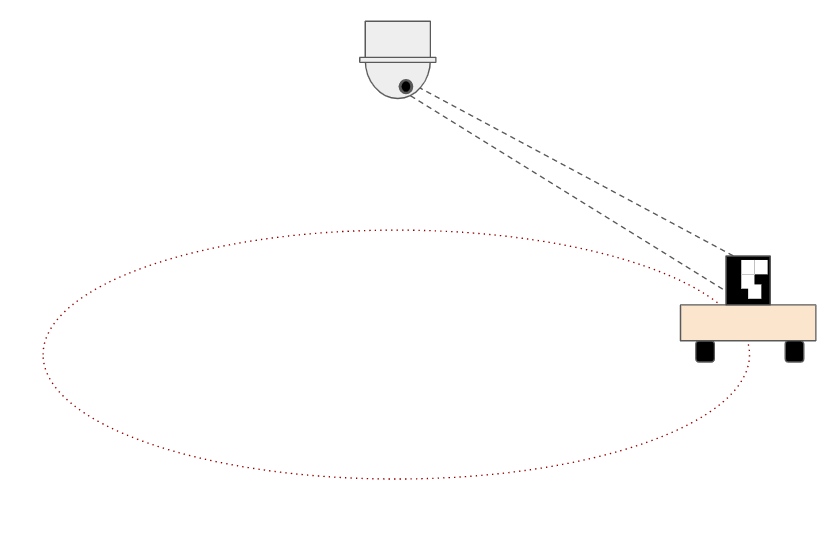
\includegraphics[width=.6\textwidth]{images/testbed2.png}
   \caption{The resulting scenario where the gimbal looks down on the Apriltag placed on top of the hoverboard.}
   \label{fig:testbed-idea-2}
\end{figure}

\subsection{Task}
The task for the operator was to keep the center of the video feed, marked with a red dot as seen in \ref{fig:interface}, aligned with the center of the Apriltag while it was moving in an ellipse inside the lab.

\subsection{Experimental Setup}
The experiment was set up in a lab where the subject and the conductor sat at a desk with a high shelf behind them, obscuring the view towards the rest of the lab. Behind the shelf, the hoverboard and gimbal boxed used were stationed. An illustration of the lab setup is provided in Figure \ref{fig:exp-setup} and a photograph of the test bed is shown in Figure \ref{fig:real-exp}.


\begin{figure}[!hbt]
   \centering
   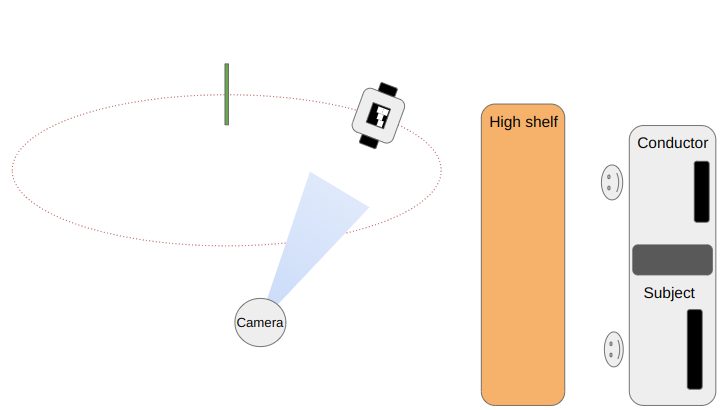
\includegraphics[scale=0.45]{images/exp-setup.png} 
   \caption{An overview of the experimental setup. To the right the experiment conductor and subject by a desk facing right. On the left side, behind the shelf, the test bed including the camera and the hoverboard are located. The camera is mounted at a height of 2.1 meters with the gimbal facing down.}
   \label{fig:exp-setup}
\end{figure}


\begin{figure}[!hbt]
   \centering
   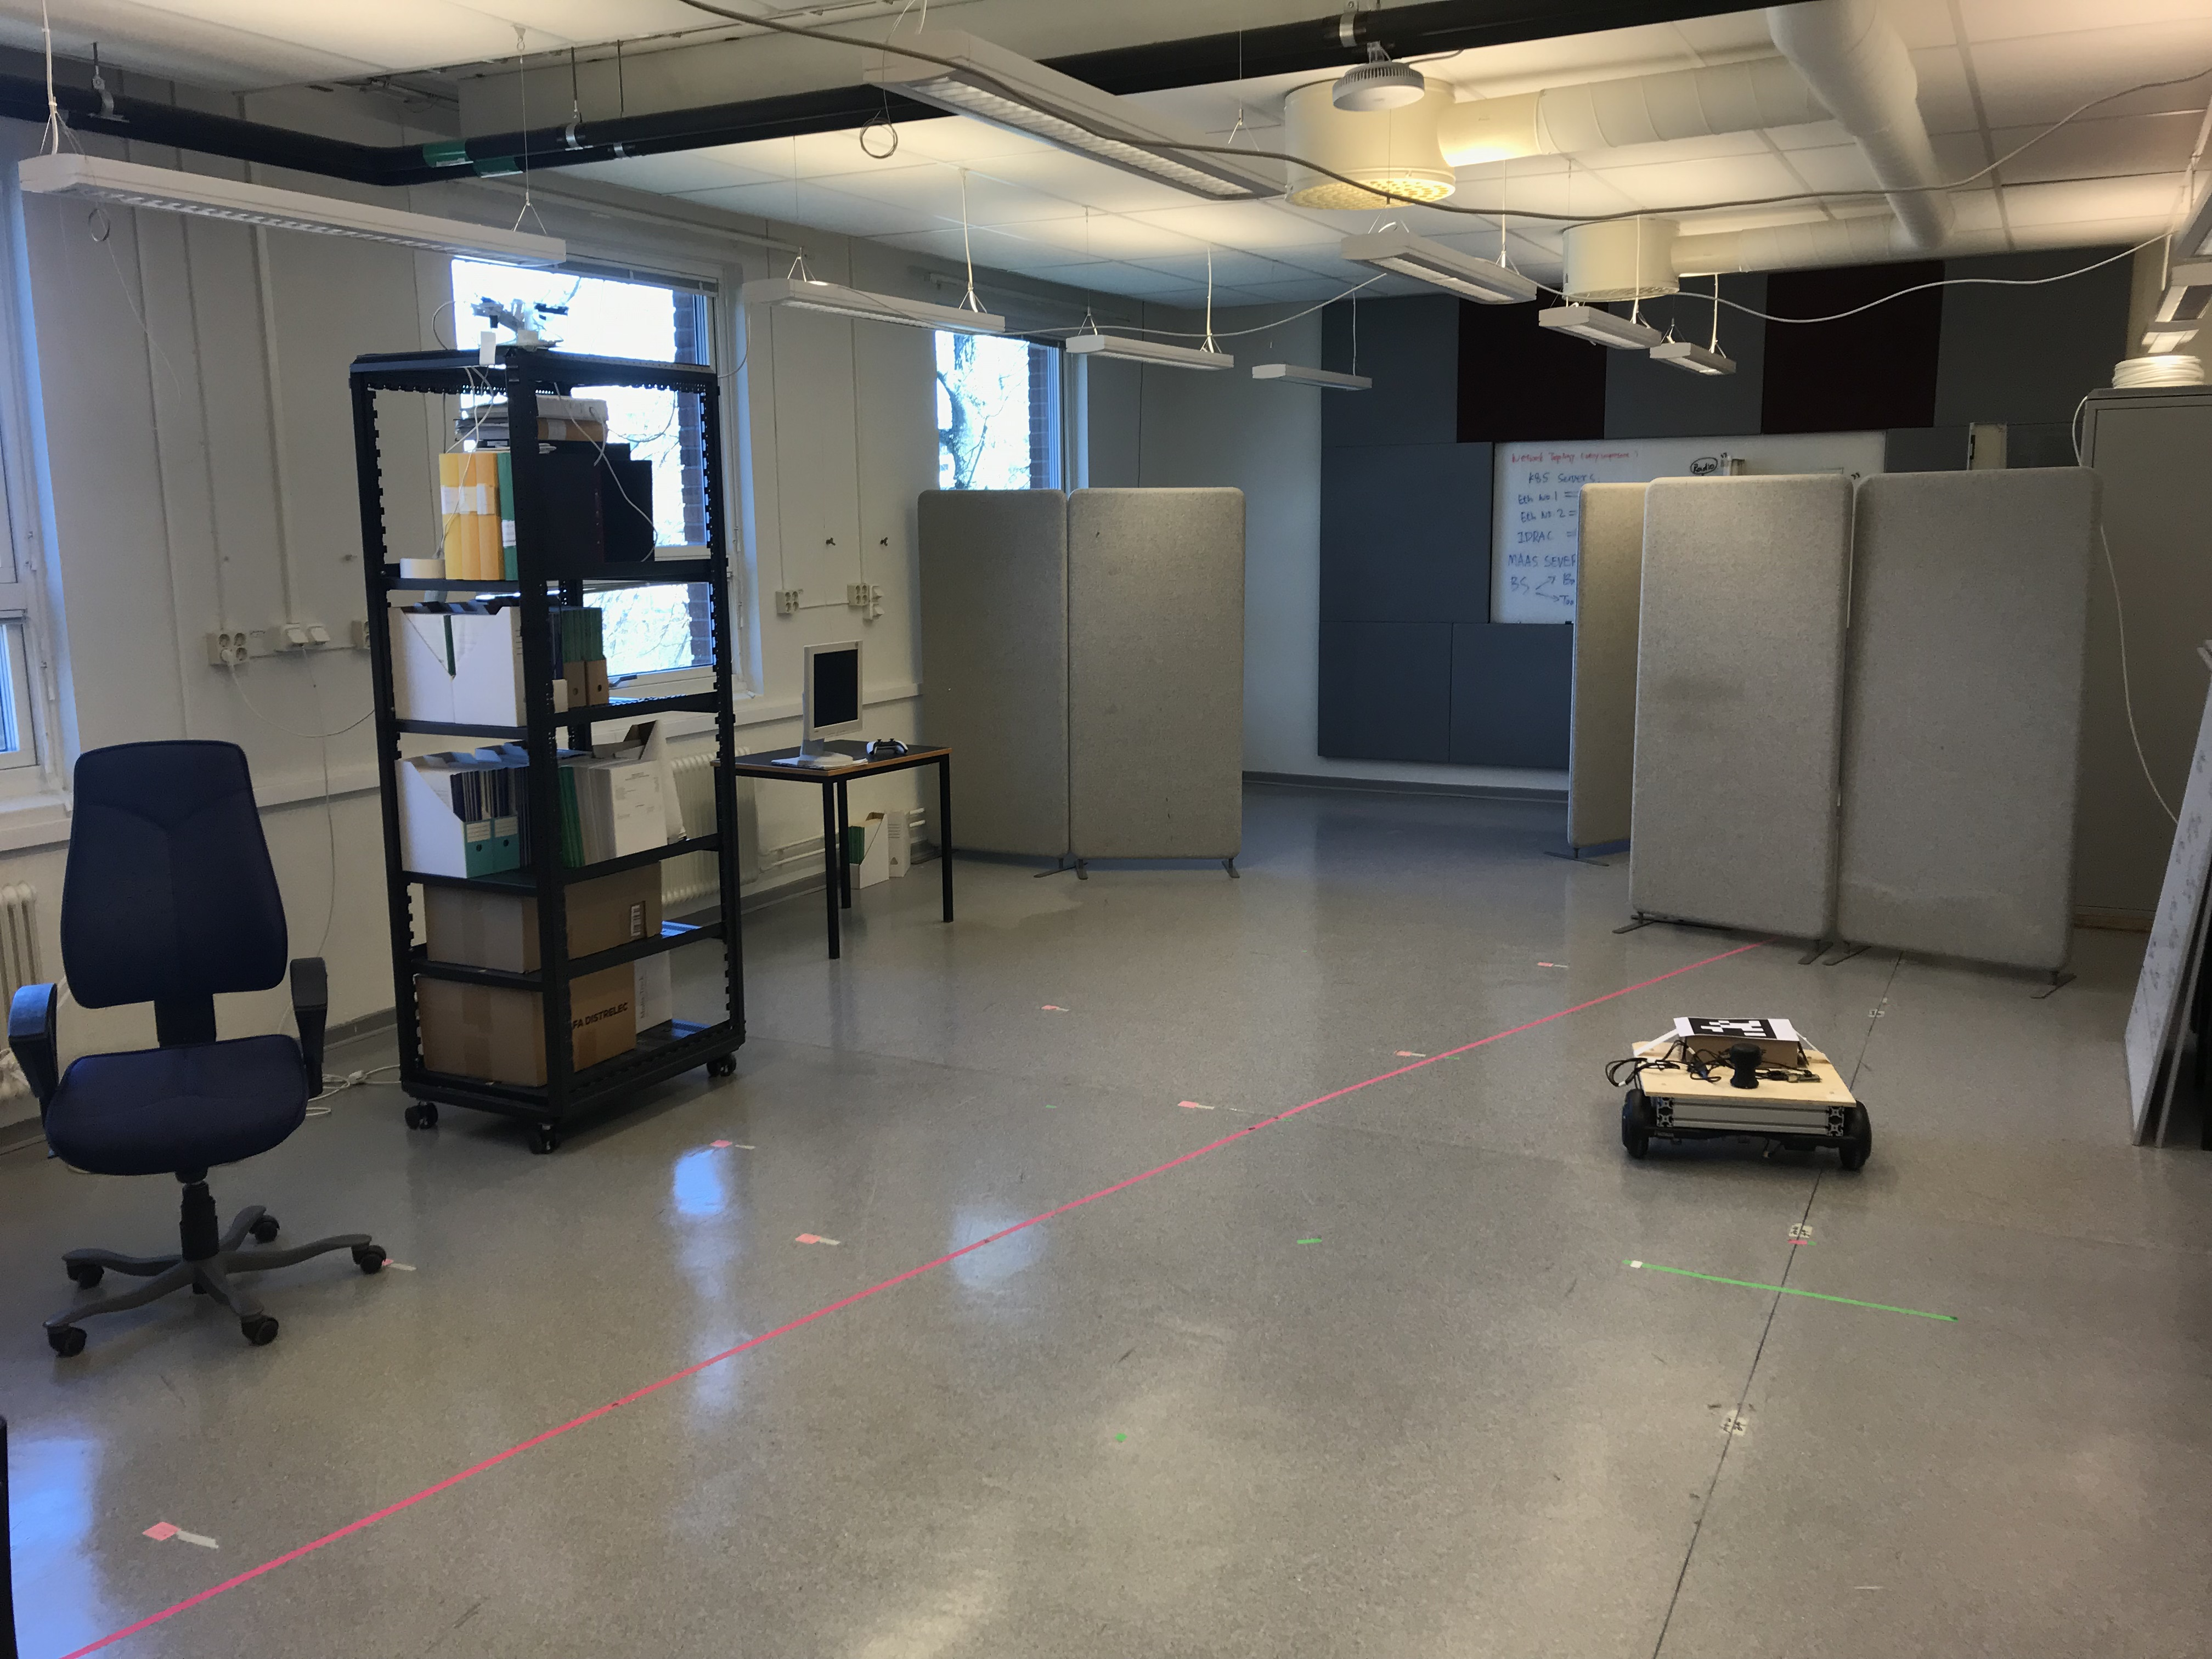
\includegraphics[scale=0.1]{images/testbed.jpg} 
   \caption{A picture of the test bed. On the left side, there is a server rack with the drone box mounted on top. The hoverboard can be seen on the right side of the picture.}
   \label{fig:real-exp}
\end{figure}

\subsubsection{Test Subjects}
The subjects were recruited mostly from the conductor's network of contacts, and for the subjects to be covered by insurance during the experiment the subjects had to be either students or employed by Lund University. Some of the participants came spontaneously while others booked a time in a spreadsheet provided by the conductor.

There was no compensation for the subjects other than home-baked goods and a hot beverage which were offered at the beginning of each experiment.

There were 10 test subjects, 4 women and 6 men, with an average age of 26.1 years where the youngest was 23 and the oldest 37. Furthermore, 5 of the subjects wore glasses and all were right-handed. 

They were also asked about their experience with games with first-person-view on the scale of 0 = None, 1 = Tried, 2 = >10h, 3 = >100h, 4 = >500h, and the median result was 3.5 with 0 as the lowest and 4 as the highest. The subjects were also asked about their experience with flying drones using the same scale, and the median result was 0.5 with 0 as the lowest and 1 as the highest. 

\subsubsection{Lab Conditions}
The lab is located in the E-building at LTH, Lund University and the windows in the room face north, so there was no risk of direct sunlight during the experiments. The computer screen was 24' and the application was run on a machine with the following specifications:
\begin{description}
   \item[CPU] Intel Core i7-4770 @ 3.40GHz, 4 cores 8 threads
   \item[RAM] 16 GB
   \item[GPU] Mesa Intel HD Graphics 4600 (HSW GT2)
\end{description}

The gimbal box was connected to the gimbal control interface via an ethernet cable as in the initial tests.

\subsection{Experimental Procedure}
In this section, each of the steps will be described in more detail. The experimental procedure is summarized in the table \ref{tab:task-timeline}.

\begin{table}[ht]
   \centering
   \caption{Task Timeline}
   \label{tab:task-timeline}
   \begin{tabular}{|c|l|l|}
   \hline
   \textbf{Time (approx.)} & \textbf{Task} & \textbf{Instruction} \\ \hline
   3 & Coffee and cookies & \\ \hline
   5 & Introduction & Tell the subject about what the study is about. \\
   & & Gather personal data + consent \\ \hline
   2 & SSQ & \\ \hline
   3 & Experiment walkthrough & What is going to happen \\
   & & Description of task \\
   & & Where to aim exactly on the Apriltag \\ \hline
   2 & Warm-up & The subject gets to try the setup for one lap \\ \hline
   10 & Tests & 5 tests with added latencies [0, 200, 300, 400, 500] \\ 
   & & in random order \\ \hline
   2 & SSQ & \\ \hline
   3 & Interview & \\ \hline
   30 & Total & \\ \hline
   \end{tabular}
\end{table}

\subsubsection{Introduction}
The experiment starts with the subject being seated at the desk to read through the consent form. After this was signed the conductor clarified that the subject was free to ask any question during the experiment and could choose to interrupt it without declaring any reason. 

Then, the subject fills out the background information form where they also get to choose a four-digit code which from that point is the only identifier of the subject and its results. If the subject booked a time slot in the spreadsheet, they were at this point removed from it.

\subsubsection{Simulator Sickness Questionnaire}
When assessing the QoE of an operator, Kennedy et. al \cite{ssq}, propose 16 symptoms that can be used to detect what is called simulator sickness. The questions are answered on a scale of 0 = "None", 1 = "Light", 2 = "Moderate", and 3 = "Severe" before the first trial and then again after the last trial. The questions are presented in Table \ref{fig:ssq-ans}.

\begin{table}[!hbt]
   \centering
   \begin{tabular}{|c|}
   \hline
   \textbf{Questions} \\ \hline
   \begin{tabular}[c]{@{}l@{}}1. General discomfort\\ 2. Fatigue\\ 3. Headache\\ 4. Eye strain \\ 5. Difficulty focusing\\ 6. Increased salivation \\ 7. Sweating \\ 8. Nausea\\ 9. Difficulty concentrating \\ 10. Fullness of head \\ 11. Blurred vision \\ 12. Dizziness (with eyes open) \\ 13. Dizziness (with eyes closed) \\ 14. Vertigo \\ 15. Stomach awareness\\ 16. Burping\\ \end{tabular} \\ \hline
   \end{tabular}
   \caption{The symptoms assessed by the subject to detect simulator sickness.}
   \label{tab:ssq-questions}
\end{table}


\subsubsection{Experiment Walkthrough}
The task was explained to the subject along with a printed Apriltag with a cross on it, indicating the spot where to aim at the tag. The particular Apriltag printed for this experiment had two white and two black squares meeting in the middle, making the center easier to identify. The Apriltag shown to the subject is shown in Figure \ref{fig:apriltag}.

\begin{figure}[!hbt]
   \centering
   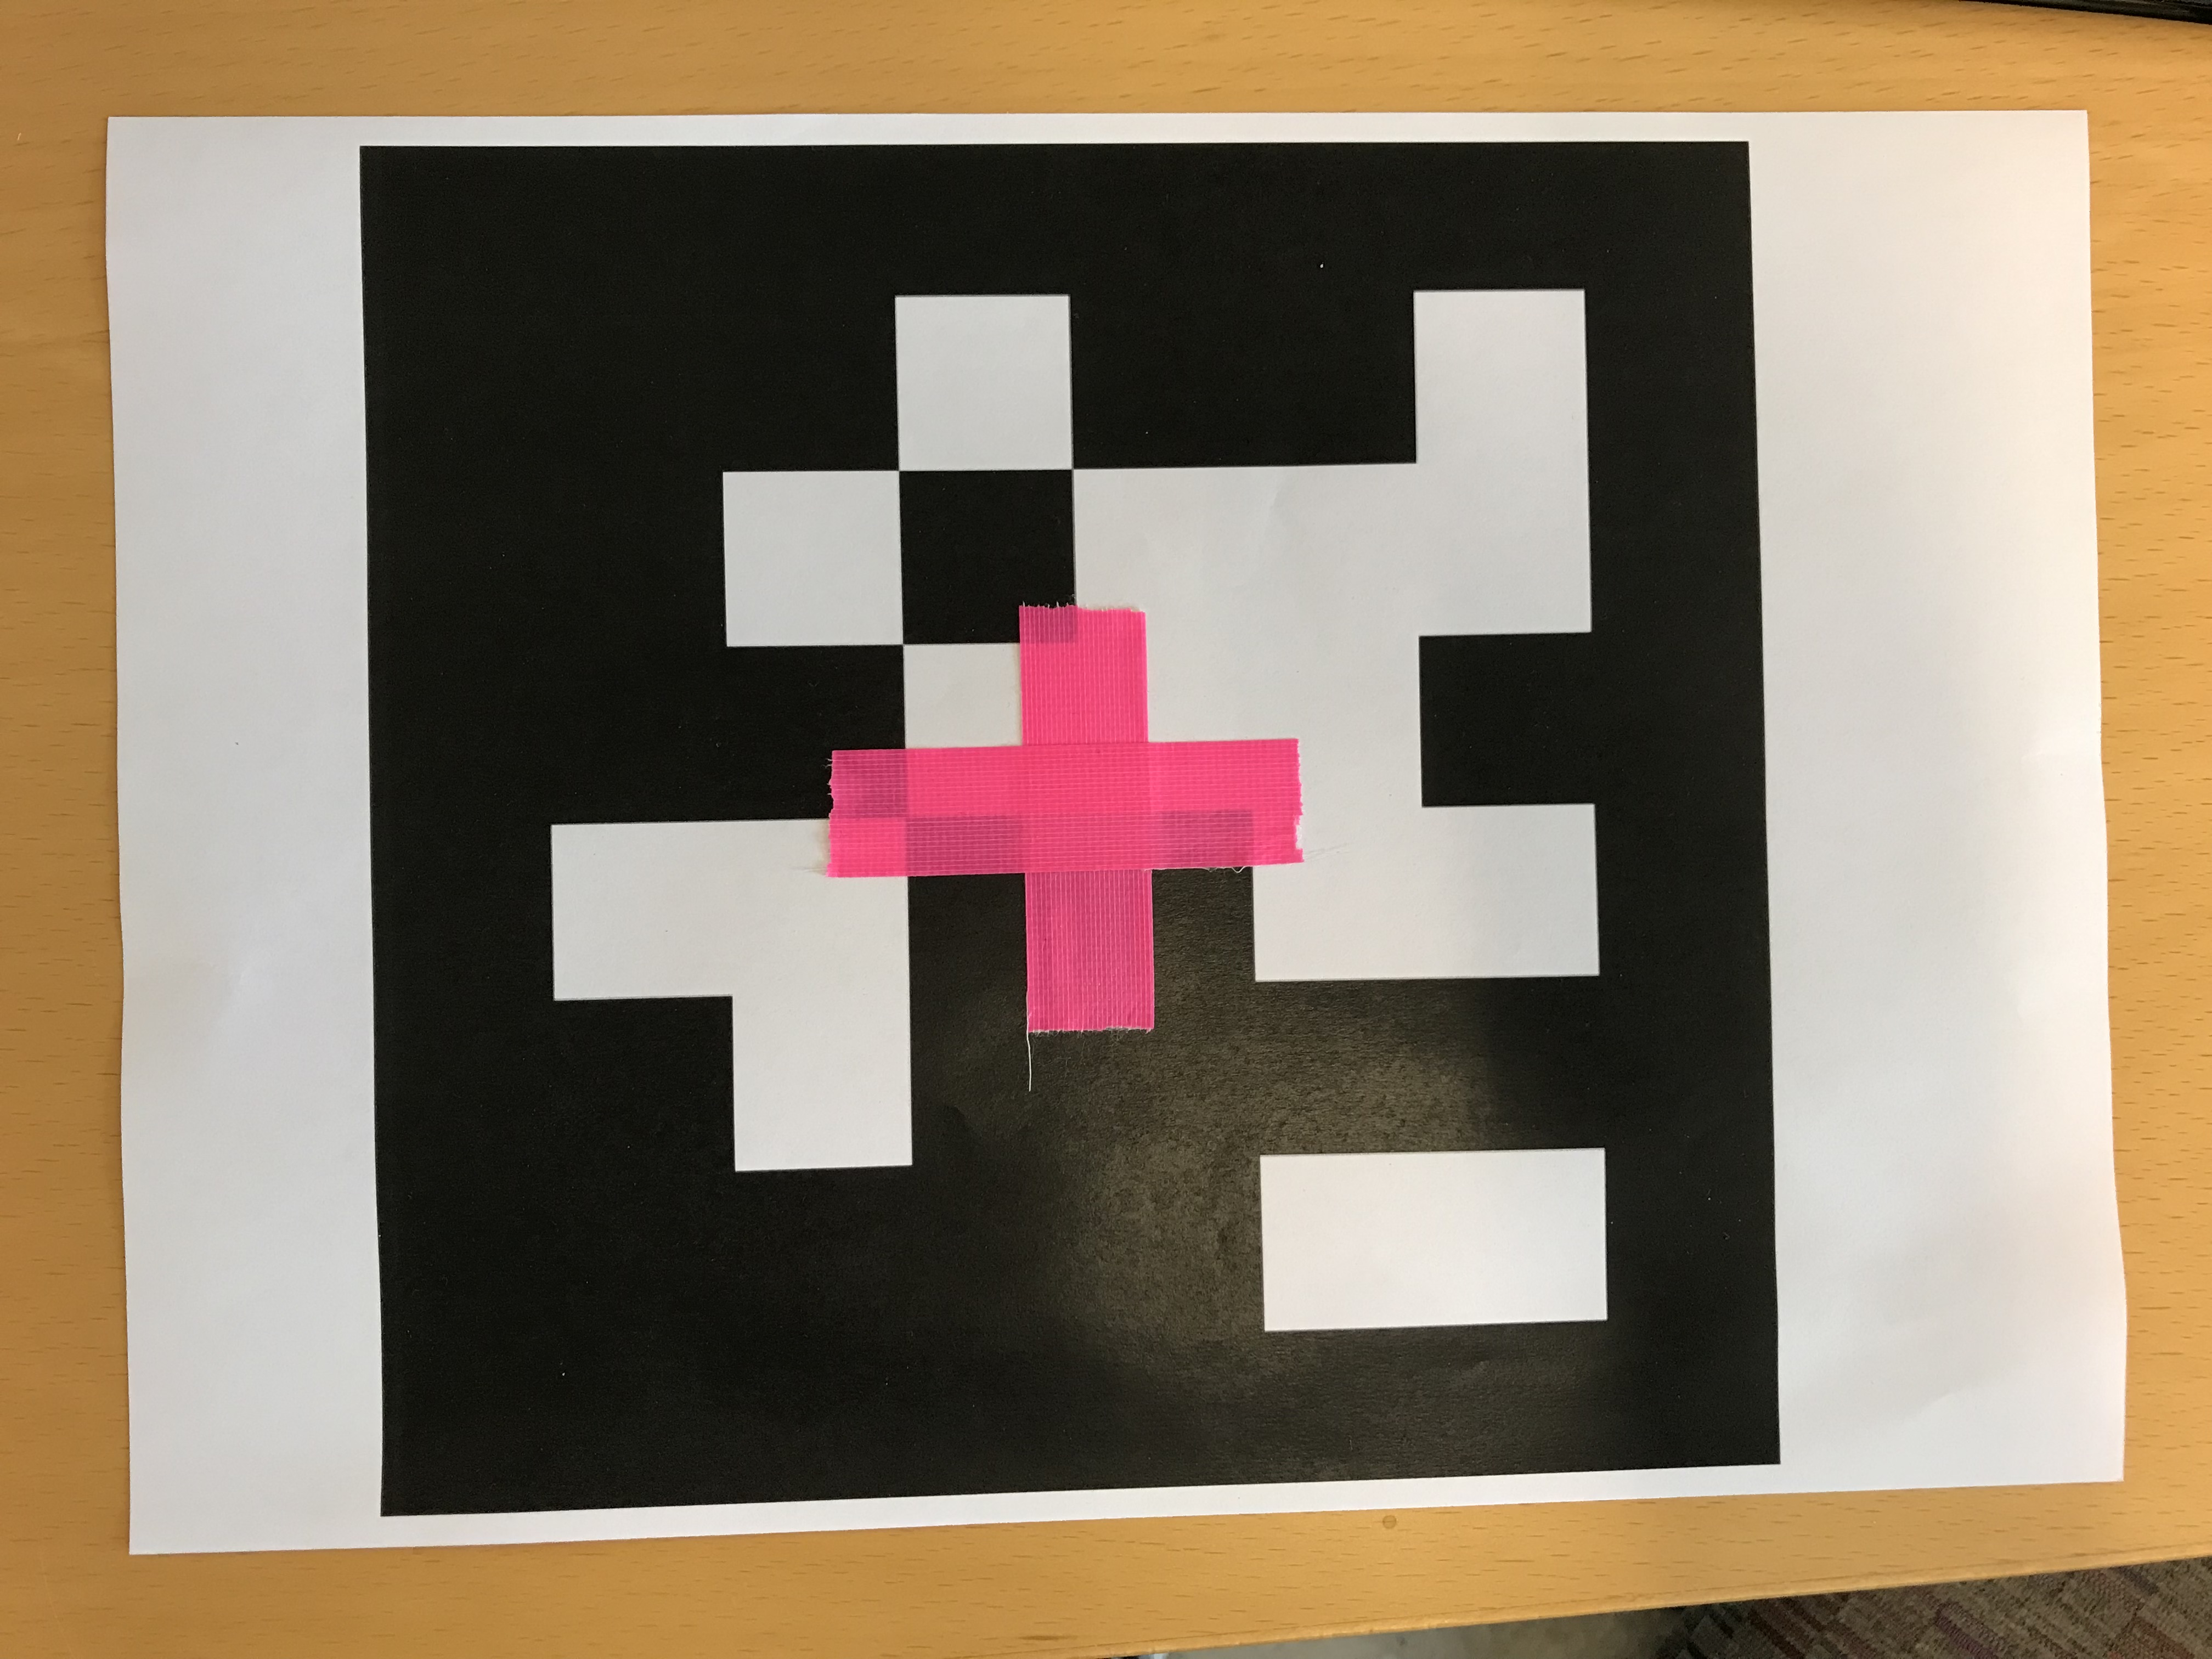
\includegraphics[scale=0.08]{images/apriltag.jpg} 
   \caption{The Apriltag used to show the subject where to aim.}
   \label{fig:apriltag}
\end{figure}

The subject was then given a chance to try the system without any delay and was given the controller and presented with the view, shown in Figure \ref{fig:interface}. The hoverboard was started and ran for one lap in the same path that it would run during the test and the subject could try and follow it.

\begin{figure}[!hbt]
   \centering
   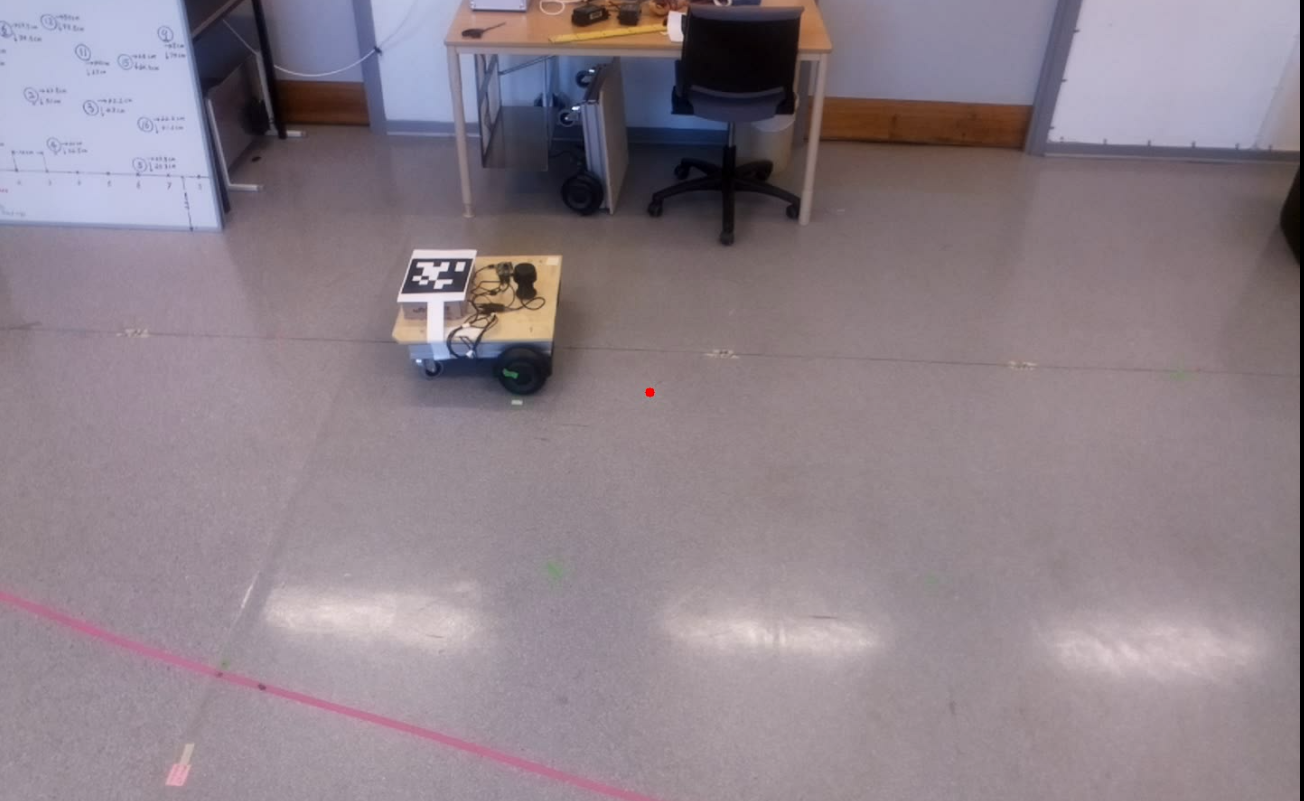
\includegraphics[scale=0.3]{images/interface.png} 
   \caption{The interface that the subject was presented with. The red dot in the middle of the screen is overlayed on top of the displayed video so that the subject has a better reference of the center of the screen.}
   \label{fig:interface}
\end{figure}

\subsubsection{Test Procedure}
After the task description and warm-up, the tests commenced. The added latencies tested were 0, 200, 300, 400 and 600 and the order in which they were given to the subject was random. 
At the beginning of each trial, the interface was restarted with one of the latencies induced in the system. The subject was then asked to put the red marker in the middle of the screen in the middle of the Apriltag. When the subject confirmed that they were ready to start the conductor started the hoverboard. The subject followed the hoverboard for two laps, which took about 2 minutes in total.

After the laps were completed the interface was shut down and the subject was asked to rate the system by answering four different questions on a scale from 1 to 5. When the subject had answered the questions the next trial was started.

At the end of the fifth and last trial, the subject got to fill in the sickness questionnaire and was also asked interview questions by the conductor.

\subsection{Evaluation}
The following two sections will describe the quantitative and qualitative methods that were used to evaluate the system.

\subsubsection{Quantitative Evaluation}
To measure the performance of each subject, the result script described in section \ref{sec:resultscript} was used. This resulted in one CSV file with about 2700 rows of data per trial. The start and end frames were extracted manually from the video of each trial and were saved in a separate file.  

\subsubsection{Qualitative Evaluation}
After each trial the subject answered a form with four questions about the system on a five-degree scale, labeled 'Terrible' to 'Excellent'. The questions are shown in table \ref{tab:form-questions}.

\setlength{\extrarowheight}{5pt}
\vspace{10pt}

\begin{table}[!hbt]
   \centering
   \begin{tabular}{|c|}
      \hline
      \textbf{How would you describe the controllability of the system?} \\
      \\
      Terrible \hspace{10pt} Poor \hspace{10pt} Fair \hspace{10pt} Good \hspace{10pt} Excellent \\    
      \\
      \hline
      \textbf{How would you rate your ability to perform the task?} \\
      \\
      Terrible \hspace{10pt} Poor \hspace{10pt} Fair \hspace{10pt} Good \hspace{10pt} Excellent \\    
      \\
      \hline
      \textbf{How pleasant was the system to use?} \\
      \\
      Terrible \hspace{10pt} Poor \hspace{10pt} Fair \hspace{10pt} Good \hspace{10pt} Excellent \\    
      \\
      \hline
      \textbf{How would you rate your impression of the system as a whole?} \\
      \\
      Terrible \hspace{10pt} Poor \hspace{10pt} Fair \hspace{10pt} Good \hspace{10pt} Excellent \\    
      \\
      \hline
   \end{tabular}
   \caption{The questions asked for each delay after each trial.}
   \label{tab:form-questions}
\end{table}

\vspace{10pt}

The interview questions can be seen in table \ref{tab:interview-questions}.

\setlength{\extrarowheight}{5pt}
\vspace{10pt}

\begin{table}[!hbt]
   \centering
      \begin{tabular}{|c|}
         \hline
         \textbf{1. What was your general experience of controlling the camera?} \\
         \hline
         \textbf{2. Did you experience any difference in the controls between the trials?} \\
         \hline
         \textbf{3. Was there any part of the track that was harder than any other?} \\
         \hline
         \textbf{4. Do you think the system would have been usable with the worst experimental conditions?} \\
         \hline
         \textbf{5. Do you think training would have helped an operator get better at using the system?} \\
         \hline
      \end{tabular}
   \caption{The interview questions asked by the conductor after the last trial.}
   \label{tab:interview-questions}
\end{table}

\vspace{10pt}

\subsection{Known Sources of Error}
\label{sources-of-error}

\subsubsection{Ecological Validity}
The future operators of the system are to be the volunteers of SSRS, which have a wide variety of ages and backgrounds. Thus, there are three main concerns with the ecological validity of the study. Firstly, the subjects were all either students or researchers at Lund University. Secondly, the average age of the subjects was low. Lastly, the sample size was only ten people. 

The first and second concerns are difficult to compensate for, as only employees or students at the university could be used as subjects due to the university's insurance. There are of course people of different ages and backgrounds working and studying at the university, but due to time restraints as well as lack of compensation for the subjects, most came from the conductor's network of contacts.

The last concern is mainly an issue with the qualitative results, as the amount of quantitative data could be increased by having each subject do several laps. Each subject generated around 13 500 data points in all five trials, resulting in about 135 000 data points for pixel error over all subjects.

\subsubsection{Frame Detection Accuracy}
The detection algorithm used to calculate the distance from the center of the Apriltag to the center of the screen could sometimes during fast camera movements not detect the Apriltag. This resulted in a NaN value at that particular frame. The average percentage of frames detected where 85\%, with a minimum of 80\% and a maximum of 89\%.

To ease the analysis of the results, all NaN values, i.e. frames where no Apriltag was detected in the frame, were linearly interpolated. To illustrate this one result is shown before and after interpolation in \ref{fig:raw-vs-interpolated}. 

\begin{figure}[!hbt]
   \centering
   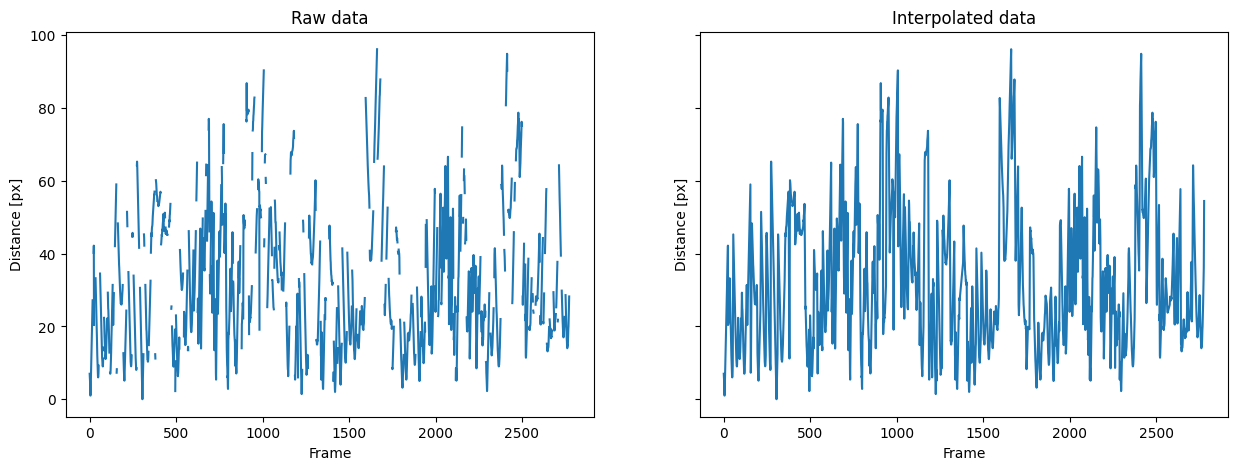
\includegraphics[scale=0.5]{images/raw-vs-interpolated.png} 
   \caption{Results for one trial: to the left the result with NaN-values and to the right interpolated result.}
   \label{fig:raw-vs-interpolated}
\end{figure}

\subsubsection{Difficulty of the Task}
The center of the Apriltag did not have a very clear center, which could have made it difficult for the subject to complete the task. To remedy this, a printed Apriltag where the center was marked out was given to the subject. However, the subject could still have had difficulty identifying the exact center of the Apriltag during the trial.

\subsubsection{Control Choppiness}
\label{sec:control-choppiness}
The control of the gimbal is done through a command sent to the drone with two angles for pitch and yaw. The drone then moves the gimbal to the desired angles. Although the angle was provided as a float, small increases from the joystick did not move the gimbal. This resulted in the control feeling choppy with the continuous input of the joystick. The choppiness also increased when looking at more distant points. 

\section{Field Testing}
The goal of this experiment was to integrate the software built for the test bed into the existing drone system, addressing goals \textbf{G3} and \textbf{G4} of the thesis scope. 

\subsection{Preparations}
For this experiment, the video and recording components were entirely removed from the GCI and the IP address to which the program connected to was changed to that of the 4G modem on the drone.

To compare the new controls to the already existing ROI mode, a button on the controller was mapped to switch between joystick mode and ROI mode, which when activated uploaded a pre-programmed GPS point for the drone to look at.

The SSRS permit to operate BVLOS in the Gothenburg archipelago requires continuous contact with the flight tower, which was initiated two weeks ahead of a scheduled flight and throughout the entire flight.

\subsection{Outdoor Conditions}
The weather was sunny with almost no clouds. The ground-level wind was estimated to be around 5-9 m/s and the temperature was around 12 degrees Celsius.

\subsection{Procedure}
A flight plan of 17 waypoints including a loiter waypoint was uploaded to the drone. The flight plan can be seen in \ref{fig:flight-plan}. The first and the last waypoints were close to the launch and the rest were placed on a route out in the archipelago. The drone was launched in manual mode and was flown in circles around the operators, confirming that all the systems were working. The drone was then switched into auto mode and the flight plan was started.

\begin{figure}[!hbt]
   \centering
   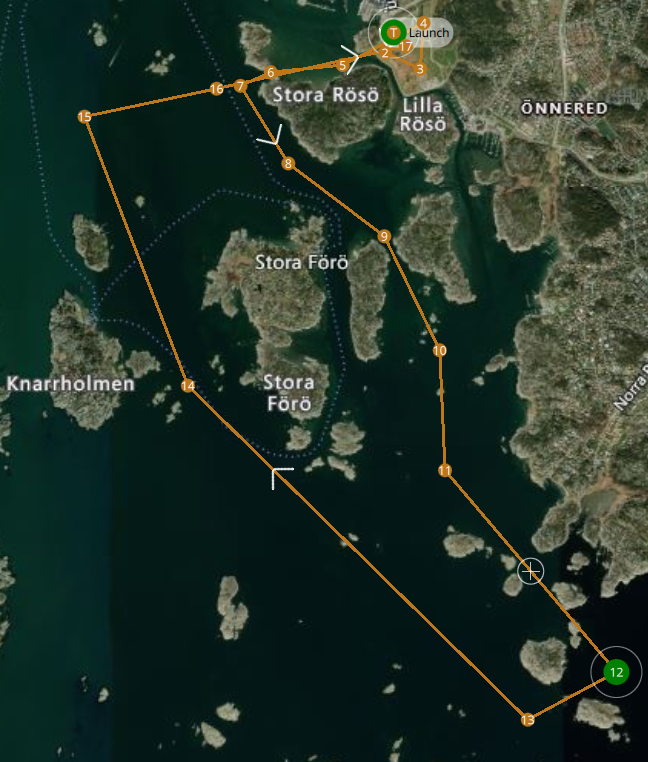
\includegraphics[scale=0.4]{images/flight-plan.png} 
   \caption{The waypoints of the flight plan. The 12th waypoint was a loiter waypoint.}
   \label{fig:flight-plan}
\end{figure}

\subsection{Delay}
During the field tests, there were several attempts of evaluating the actual latency of the drone by measuring pings and comparing the on-board system clock to the time on the ground station. However, the results were inconclusive and the latency could only be estimated.

\chapter{Results}
This chapter will go through the main findings of the two experiments.

\section{QoE Experiment}
In this section, the results from the QoE experiment are presented.  

\subsection{Quantitative Measurements}
To ease the interpretation of the results, two examples of different pixel errors of 48 and 178 are shown in Figure \ref{fig:pixel-error}. 

\begin{figure}[htp]
   \centering
   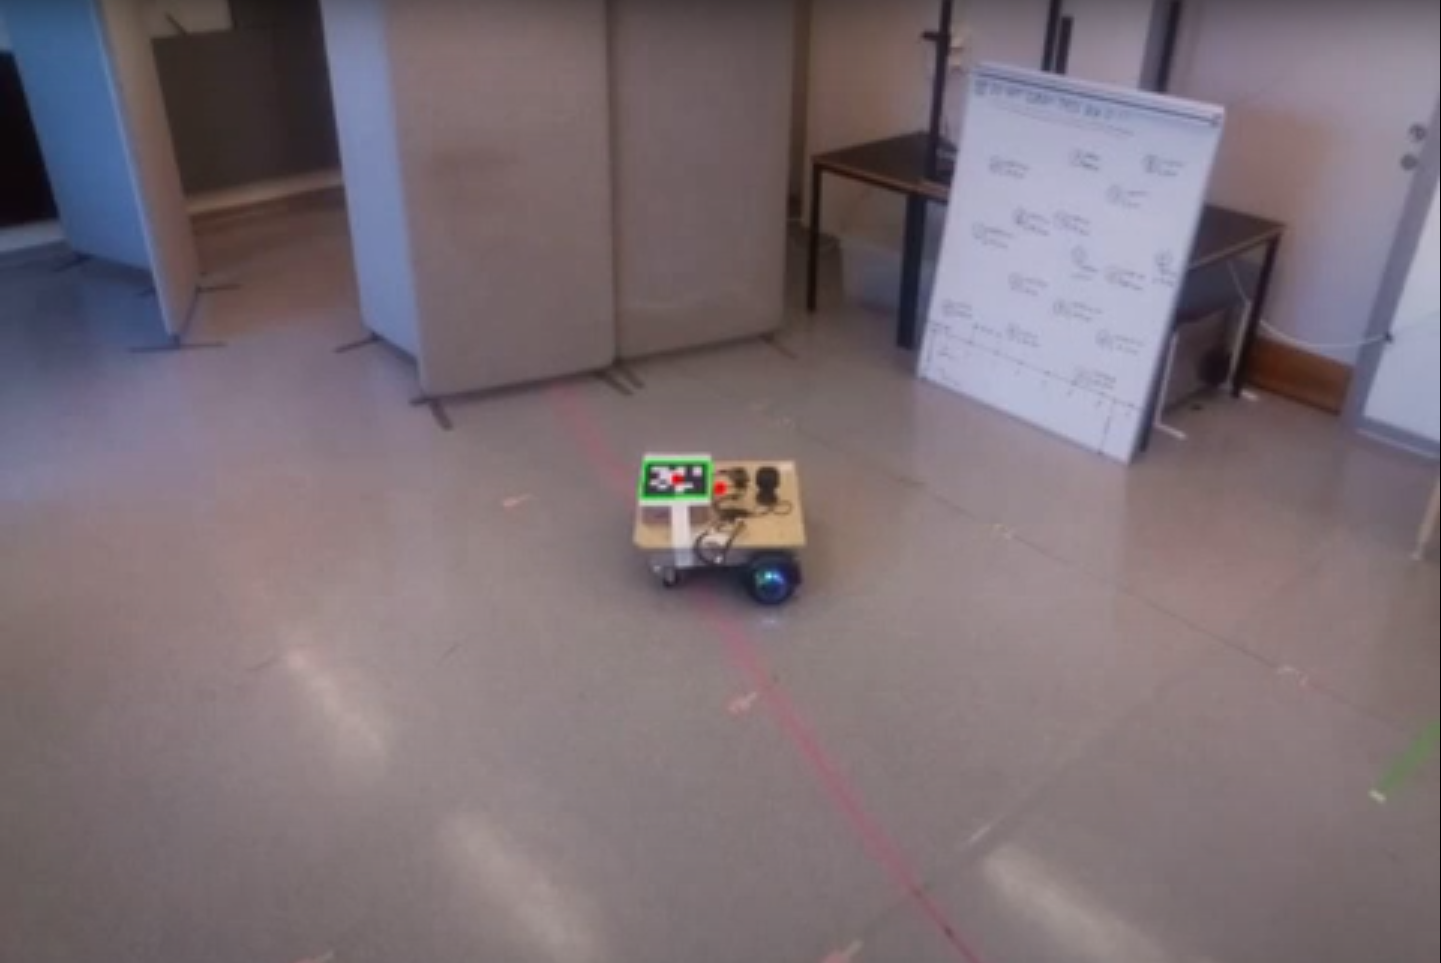
\includegraphics[width=.47\textwidth]{images/pixel-error-low.png}\hfill
   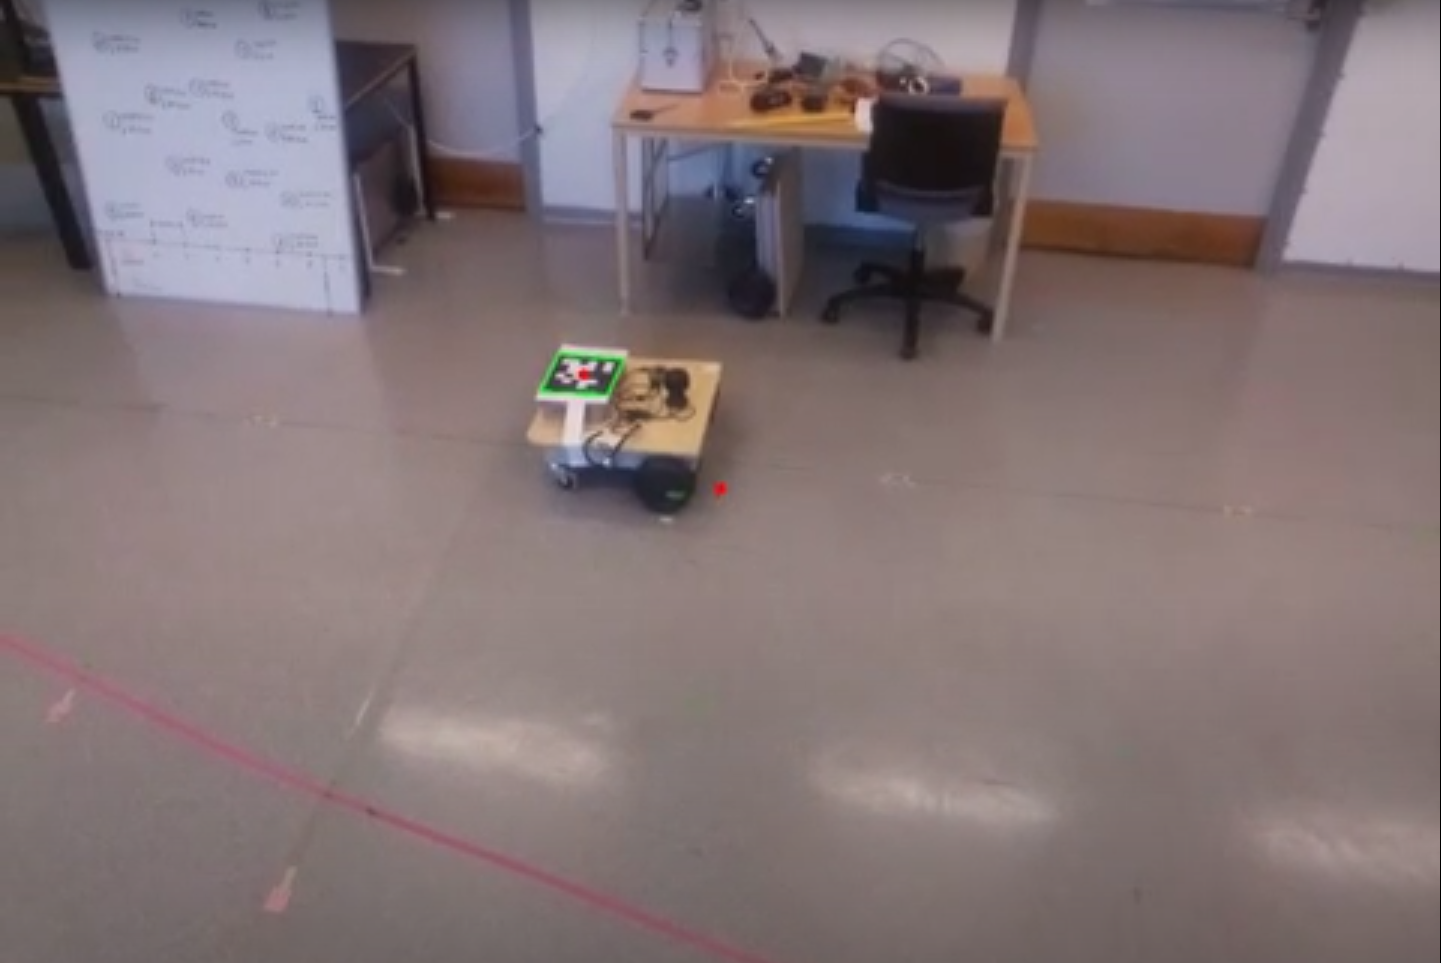
\includegraphics[width=.47\textwidth]{images/pixel-error-high.png}
   \caption{Examples of two pixel errors from a trial. In the leftmost picture the pixel error is 48 while in the rightmost picture, the pixel error is 178.}
   \label{fig:pixel-error}
\end{figure}

In \ref{tab:averages} the mean and standard deviation of the different delays are presented when averaged over all subjects. The values are also visualized in plot \ref{fig:avg-std}. A clear trend can be seen where both the mean and standard deviation increase with the delay. An interesting feature of the data is that the mean after 400ms starts to increase at a non-linear rate, while the standard deviation has a more or less linear increase throughout the added delays.

\begin{table}[ht]
   \centering
   \begin{tabular}{|c|c|c|}
   \hline
   \textbf{Delay} & \textbf{ Mean (ms)} & \textbf{Std. deviation (ms)} \\
   \hline
   0 & 29.8 & 18.0 \\ \hline
   200 & 35.2 & 22.3 \\ \hline
   300 & 41.5 & 26.8 \\ \hline
   400 & 46.0 & 28.7 \\ \hline
   600 & 61.8 & 37.2 \\ \hline
   \end{tabular}
   \caption{Means and standard deviations for the added delays.}
   \label{tab:averages}
\end{table}


\begin{figure}[!hbt]
   \centering
   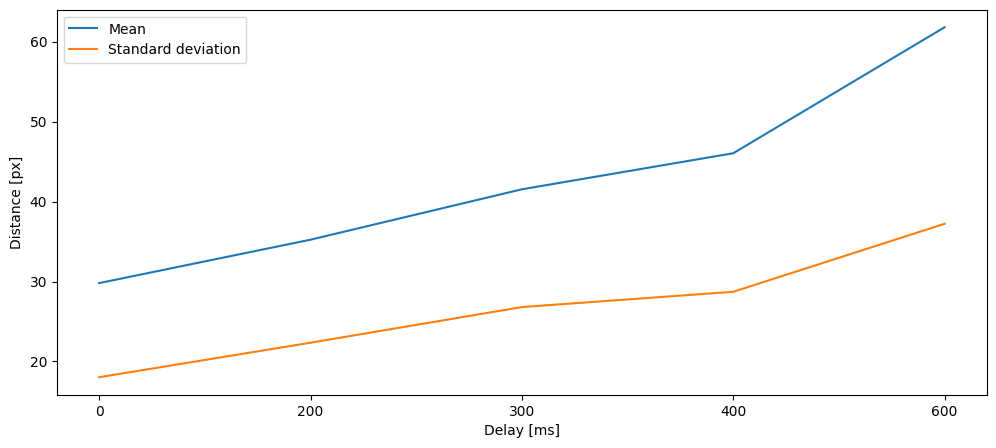
\includegraphics[scale=0.5]{images/avg-std.png} 
   \caption{Pixel error average and standard deviation for all delays. Delays 100 and 500 are added on the x-axis for the correct scale.}
   \label{fig:avg-std}
\end{figure}

In figure \ref{fig:ecdf} the empirical cumulative distribution functions (ECDF) for the results of each delay are shown. The x-axis represents the value that the entry has while the y-axis represents the percentage of entries that are less than or equal to the x-axis value. The increase in both the average and mean can be observed as the delay increases. It can also be deduced that the distance between the curves 0ms and 200ms is much smaller than that between the curves 400ms and 600ms. This could indicate that the additional 200ms added delay had a larger impact at 400ms than at 0 ms.

When taking into account the inherent latency of the system of around 400ms, there seems to be a larger effect on operator performance at the only latency higher than 800ms. This was also the threshold delay for which an observable effect on controller latency was found in \cite{latency-impact}.

\begin{figure}[!hbt]
   \centering
   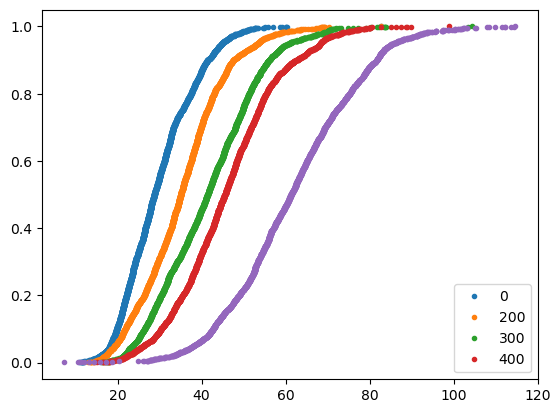
\includegraphics[scale=0.5]{images/ecdf.png} 
   \caption{ECDF of the total pixel error averaged over all subjects. The curves show the distribution of the error for each delay. A larger inclination suggests a larger spread and the more to the right the curve is, the larger the average error.}
   \label{fig:ecdf}
\end{figure}

In Figure \ref{fig:hoverboard-pos} all the values from the trials have been averaged and the position of the hoverboard has been superimposed, where one period represents one lap. In this plot, one can see that the final corner of the track is the most difficult and that the very end and early beginning of the track are the easiest. 

\begin{figure}[!hbt]
   \centering
   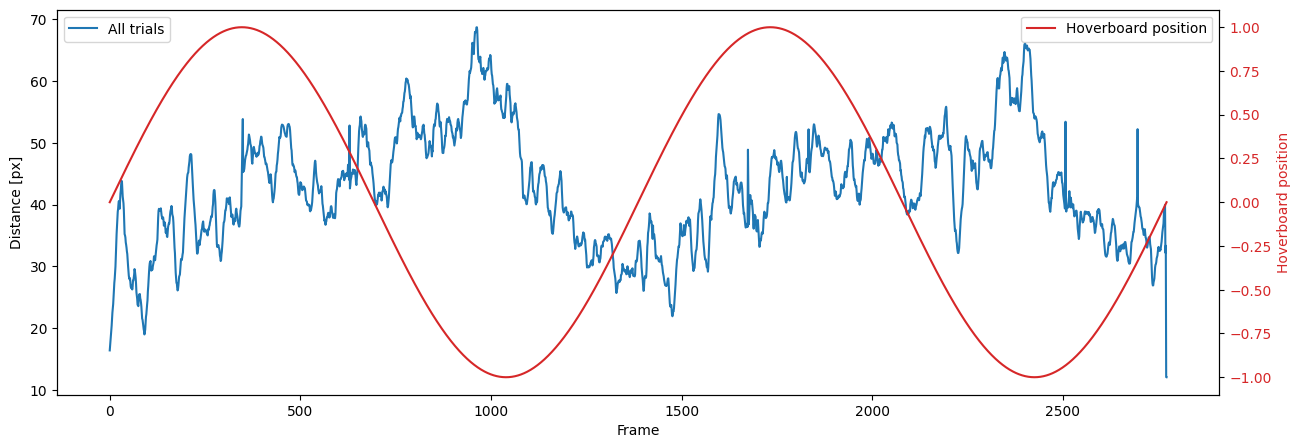
\includegraphics[scale=0.4]{images/hoverboard-pos.png} 
   \caption{All trials averaged with hoverboard position superimposed. The error steadily increases up until the end of the last corner where it decreases rapidly.}
   \label{fig:hoverboard-pos}
\end{figure}

In Figure \ref{fig:0vs600}, the results from 0ms and 600ms are shown with the hoverboard position superimposed. The more transparent blue and green lines represent the average over all trials while the darker lines are a rolling average of the data. The red line represents the position of the hoverboard. Here, both the increase in mean and deviation are visible. 

\begin{figure}[!hbt]
   \centering
   \makebox[\textwidth]{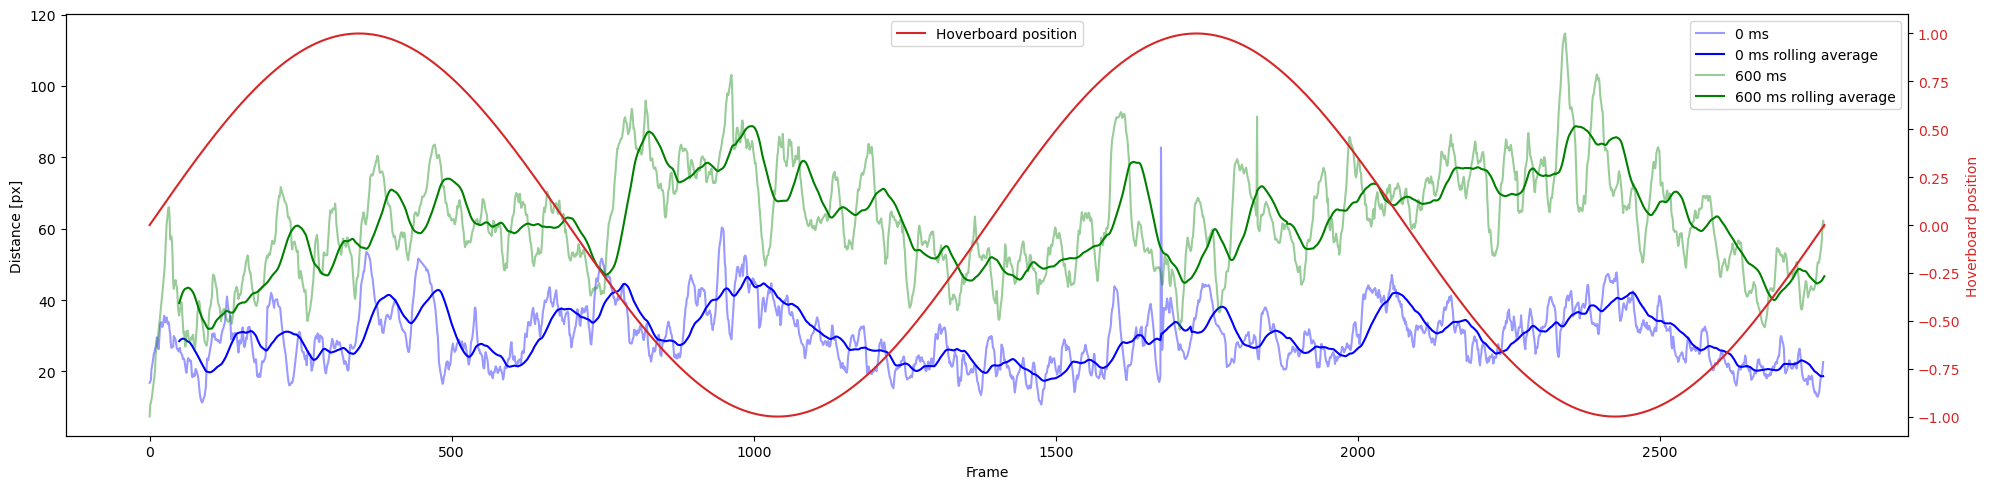
\includegraphics[scale=0.35]{images/0vs600.png}}
   \caption{Total trials for latencies 0 and 600 averaged over all subjects with hoverboard position superimposed.}
   \label{fig:0vs600}
\end{figure}

In Figure \ref{fig:indv-perf} the distributions of the test subjects' results on each delay are shown. By comparing the best and worst performance at each delay, it can be seen that the worst performance increases much more than the best performance. This suggests that an operator's skill is more important at higher delays. 

\begin{figure}[!hbt]
   \centering
   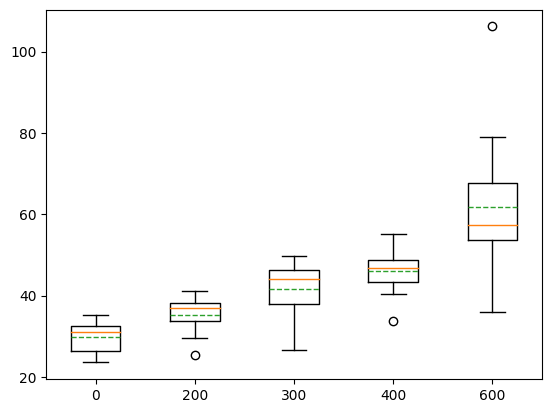
\includegraphics[scale=0.8]{images/indv-perf.png} 
   \caption{The distribution of the individual results for each delay. The lower ends of the plot represent the best performance at that added latency while the upper ends represent the worst performance.}
   \label{fig:indv-perf}
\end{figure}

\subsection{Forms and Interviews}
In this section, the results from the forms and interviews are presented and discussed.

\subsubsection{Trial Forms}
As only 10 subjects completed the trials the answers from all the questions on each delay were grouped, making for 40 answers on each delay. A box plot showing the distributions of the answers is shown in \ref{fig:form-ans}. For one subject, the 200ms trail was forgotten and was instead filled with the average answer 3 for all questions afterward.

Looking at the averages a clear downward trend can be seen with an increase in delay. The largest differences in score are between 0ms to 200ms and 400ms to 600ms, which is to be expected with the larger steps in delay. However, the trend does not seem to correspond to that of the quantitative results in \ref{fig:ecdf} where the step from 0ms to 200ms is about the same as between 200ms, 300ms and 400ms. Although there is a trend in the average, the distributions seen in \ref{fig:form-ans} are quite similar, and more trials and delays are necessary to deduce an exact connection between task performance and operator experience.   

\begin{figure}[!hbt]
   \centering
   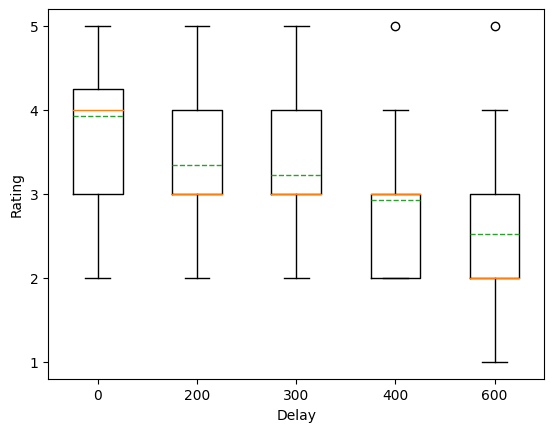
\includegraphics[scale=0.6]{images/form-ans.png} 
   \caption{Box plot of form answers for each delay. The green line represents the mean while the orange line represents the median.}
   \label{fig:form-ans}
\end{figure}

\subsubsection{Simulator Sickness Questionnaire}
In \ref{fig:ssq-ans} the difference in SSQ answers before and after the trials has been averaged over all subjects. The largest response increase is on symptom four, namely "eye strain", which had an average increase of 0.5 with four out of all the subjects reporting an increase. The next two highest symptoms were "fullness of head" and "blurred vision". 

The results from the SSQ suggest a small increase in symptoms after the trials, but the increase is not large enough to be considered significant for a sample size of only 10 subjects.

\begin{figure}[!hbt]
   \centering
   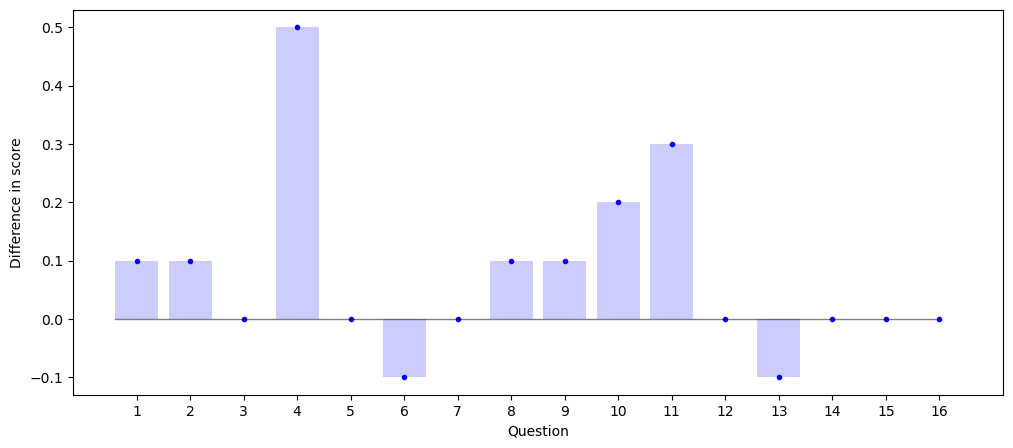
\includegraphics[scale=0.6]{images/ssq-results.png} 
   \caption{Difference in SSQ answers from before and after the trials on a scale from 0 to 4.}
   \label{fig:ssq-ans}
\end{figure}

\subsubsection{Interviews}
The answers to the interview questions will be summarized in this section.

\titleformat{\paragraph}[hang]{\normalfont\small\bfseries}{\theparagraph}{1em}{}
\titlespacing*{\paragraph}{0pt}{3.25ex plus 1ex minus .2ex}{1em}

\paragraph{1. What was your general experience of controlling the camera?}
A majority of the subjects reported that camera controls felt choppy, which is probably caused by the controls, explained in section \ref{sec:control-choppiness} on control choppiness. The subjects also reported that the controls felt very different throughout the trials. Some subjects also said that they grew more accustomed to the controls as the trials progressed.

Some quotes from the subjects are presented below.
\begin{description}
   \item[Subject 4545] "Had this been my day job I would have jumped out the window". 
   \item[Subject 1111] "Intuitive, sometimes there was delay that made it difficult."
\end{description}

\paragraph{2. Did you experience any difference in the controls between the trials?}
All the subjects felt reported a difference in the trials. Usually, subjects had a clear view of which trials were the easiest or the most difficult.

\paragraph{3. Was there any part of the track that was harder than any other?}
Almost all subjects reported that the last corner was the most difficult out of the entire track. This is supported by the quantitative results, as a visible spike shows in the average over all subjects.

Some also stated that it was easier when the hoverboard was closer to the camera. This could be due to the effect of the gimbal's choppiness which was less noticeable at short range, as explained in section \ref{sec:control-choppiness}.

One possible explanation for the difficulty of the upper right corner would be that the hoverboard was moving diagonally away from the camera, which would make it harder to follow as the choppiness led to discrete movements.

\paragraph{4. Do you think the system would have been usable with the worst experimental conditions?}
On this question, the answer of the subjects varied. A couple gave an absolute no, while others said that it depended on how precise one had to follow the object. 

\paragraph{5. Do you think training would have helped an operator get better at using the system?}
All the subjects responded that training would improve one's performance in the system and that they got better at the task as the trials progressed. 



\section{Field Testing}
Before the test flights, the GCI was successfully integrated into the running system and was shown not to interfere with the pilot controls. Thus, goal \textbf{G3} was reached.

During the flights, the two different modes of operation were tested and the results are presented in the following sections.

\subsection{Manual Control}
During the initial loiter, the plane's orientation changed a lot due to the incoming angle of the wind constantly changing. This made the gimbal very difficult to control manually, with the delay of the controls making it almost impossible to compensate for sudden movements, for example when the plane made an aggressive roll or yaw.

After the plane had left the initial loiters it had more time to fly straight. During this time the camera was much easier to control manually, as the plane was more stable and the orientation remained the same for longer. 

Between waypoints 11 and 12, a boat was spotted coming up beside the drone which the gimbal operator decided to try and follow. Although considerable delay made it more difficult to control the gimbal than in the lab experiment, the boat was successfully followed for around three minutes. An illustration of the event can be seen in \ref{fig:boat-follow}. It was observed that the operator could predict the position of the boat, allowing preemptive gimbal movements to compensate for the delay. 

\begin{figure}[htp]
   \centering
   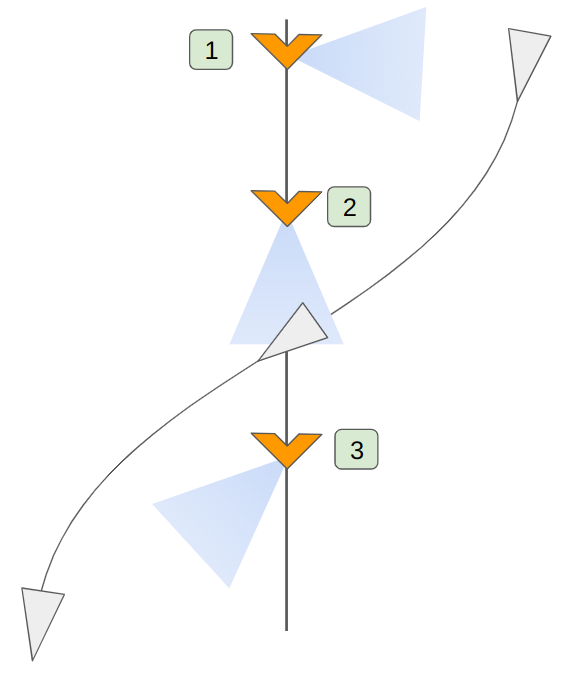
\includegraphics[width=.5\textwidth]{images/drone-boat-illustration.png}
   \caption{Illustration of the drone following the boat (not in real scale). The orange shape represents the drone and the grey triangle represents the boat. The green boxes indicate points in time and the blue cone is the drone's field of view which was changed by the GCI during flight.}
   \label{fig:boat-follow}
\end{figure}

Another observation from the experiment is that being a fixed-wing aircraft, the operator's ability to control the camera relies heavily on the position and heading of the aircraft. This means that in a real scenario, the operator's ability to control the camera would be dependant highly dependent on the controls of the aircraft. 

\subsection{ROI Control}
The ROI mode was activated on waypoint 12 and worked well when the drone was turning at a shorter radius. However, there were some inconsistencies in the altitude data for the points which caused the camera to point at a point below the surface of the earth. The point was adjusted by raising the altitude parameter of the ROI. 

It could also be observed that increasing the loiter radius gave a better image as the inexactness of the GPS point was less impactful. 

\chapter{Discussion}
In this chapter, a comparison between the GCI and the state-of-the-art will be made. Then, the work's impact, limitations, weaknesses, and strengths will be discussed. Finally, its contribution will be analyzed from a sustainability and ethics perspective.

\section{Comparison with State-of-the-Art}
In this section, a comparison with other modern systems will be made. First, the QoE test bed is compared to other ones within the research field. Then, the specific functionality, namely gimbal control, is compared to already existing solutions in the commercial, military and DIY sectors.

\subsection{QoE Test Bed}
During the development of the test bed, the research facility RISE (Stockholm, Sweden) was contacted as they had ample experience conducting QoE experiments. During the time of the thesis' work, valuable insights and suggestions were conveyed through several meetings with Kjell Brunnström. A visit was also made to their offices where I got the chance to be a subject in one of their QoE experiments conducted by a PhD student. Although the experimental conditions and objects of study were different, the test beds shared many similarities. 

\subsection{Commercial Systems}
In the drone consumer market, the Chinese manufacturer DJI holds a global market share of more than 70\%, according to CNBC \cite{dji}. Their most popular systems are targeted toward filming and a lot of them feature camera gimbals with features such as stabilization, target following and ROI mode. 

For companies or hobbyists building drones, there are also separate drone gimbals that can be bought from manufacturers such as Gremsy \cite{gremsy} or SIYI \cite{siyi}. These particular gimbals cost \$1,399 and \$529.42 respectively and their functionality is highly dependent on the onboard software. For comparison, the SSRS gimbal can be assembled for approximately \$50 with off-the-shelf components and a 3D printer.

\subsection{Military systems}
As fixed-wing UAVs with gimbals have seen heavy use in the military sector, a high level of sophistication in UAVs and their operations is usually found in these types of systems. One of the most historically known military drones also featuring a camera gimbal is the MQ-9 Reaper \cite{mq9reaper}, which saw heavy use by the U.S. during the conflicts in Iraq and Afghanistan \cite{mq9reaper-wiki}. More modern systems with drones in more similar size to the SSRS drone (although with very different use cases) include the Turkish Bayraktar drones \cite{bayraktar-wiki} as well as the Switchblade series \cite{switchblade} from the American company AeroVironment.

\subsection{ArduPilot Ecosystem}
In the ArduPilot ecosystem, gimbal control has seen much development in the last year, with the command used for the functionality in this thesis being supported only since the summer of 2022 \cite{ardupilot-gimbal-issue}. As this feature is so new in the drone's onboard software it has not yet been integrated into the mission control software, making it inaccessible for those without the know-how to create an interface themselves.

\section{Impact}
The test bed developed in this thesis shows promise for evaluating different parameters relevant to QoE research. Beyond further research, the software will be used as a starting point for gimbal control in the SSRS mission control software, contributing to the development of modern SAR tooling. Their system could also be extended to other domains where UAVs have been investigated such as SAR in mountain environments \cite{drones-mountain-sar} or wildfire monitoring \cite{drones-wildfire}.

\section{Limitations}
The main limitation of the test bed is that the scenario keeps the drone stationary, which is not the case in real flight. Although the results from the experiment are interesting in their own right, the scenario in the experiment is not analogous to that of a real SAR operation. This is mainly due to the experiment only being limited to one scenario where the hoverboard ran in a predictable path, making the results not generalizable to all paths and scenarios.

In the real flight scenario, conducting controlled experiments was limited due to various factors. The primary obstacle lies in the extensive preparations required for each mission, where setting up the drone and its intricate systems demands substantial effort and time. Furthermore, numerous regulations and safety measures must be adhered to before undertaking an unmanned BVLOS flight. For example, communication with air traffic control about the mission is initialized two weeks before the flight, and contact is held during the entirety of the mission.

Due to the scarcity of actual flight tests, gimbal control was usually not the main goal of the flight, which meant that there were limited possibilities to set up scenarios to evaluate operator performance in the system during flight. One example of this is the so-called "earth-frame"-mode, with which the gimbal points in a compass heading instead of an angle relative to the aircraft. This effectively stabilizes the yaw-axis as well which could improve the steering sensation when flying. Due to time limitations, this mode was not tested but could be of interest in further research.

An initial wish was also to have the software contributed back to the ArduPilot ecosystem, which was unfortunately not possible as time did not allow for the software to be developed to a sufficient level of quality.

\section{Weaknesses}
For the QoE experiment, the main sources of error are presented in their entirety in section \ref{sources-of-error}. Among these, the most significant is probably the feeling of the controls, as many subjects reported on this in their interviews. Furthermore, the subject had no say in the sensitivity of the controls or if they preferred to use a different control scheme.

A big weakness is also the subject selection, as they were not representative of society as a whole nor the target group of the future SSRS system. There were only 10 test subjects, and as the results indicate a large variance in performance between the test subjects, individual performances could have a large impact on the results. Nevertheless, training in the system can be expected to improve an operator's ability to compensate for delays. 

In regards to flight testing, the main goal of the thesis was to have working controls and it was uncertain whether a test scenario would be possible to set up. As a result of this, the in-flight tests of the gimbal, albeit successful, are not so generalizable. 

\section{Strengths}
The test bed along with the evaluation method presented in this thesis is a novel approach to QoE experiments, where qualitative measurements can be taken in high quantity unintrusively to the test subject. Due to the design of the ArduPilot ecosystem, the test bed is also compatible with other ArduPilot systems and would require no modification to work on other vehicles such as multi-rotors, rovers or even submarines.

Another strength of the thesis work is that the software was robust enough to be used in a real flight scenario and will be used in future flight testing.

\section{Sustainability}
As the UAV is electrically powered, it does not produce any direct CO2 emissions during use. Considering future SAR scenarios, early imagery could allow a rescue crew to go at lower speeds, reducing engine emissions as well as the boat's effects on the surrounding environment. 

Currently, helicopters or airplanes can be put in for aerial support during SAR missions. In the future, drone systems could support or in some instances completely replace these manned vehicles, and with their smaller size and electrical propulsion they would have much smaller CO2 emissions.

\section{Ethics}
The software implemented in this thesis is aimed at assisting in SAR operations and its functionality can as such be deemed critical to human life. Although the idea is that aerial imagery is only to be used as support, the intelligence provided by said imagery has to be reliable as it can affect the decisions onboard a rescue vehicle. This places higher requirements on the robustness of the system and its' operator. 

Although the software developed for this thesis is aimed at a certain type of operation, gimbal control remains highly applicable to more ethically questionable tasks such as surveillance or target acquisition for weapons. 

In a discussion in the ArduPilot forums \cite{ardupilot-military-discussion}, a user provides an image of the software Mission Planner (a GCS in the ArduPilot ecosystem) being used in what seems to be a military operation. Although ArduPilot states in their code of conduct \cite{ardupilot-coc} that they pledge to not support or facilitate the weaponization of systems based on their software, the accessible nature of it enables anyone to use it for any purpose. In research alone, numerous examples can be found \cite{ardupilot-military} \cite{ardupilot-military-1} where parts of the ArduPilot software and hardware ecosystem are used in military settings.

Despite this evidence, the nature of open source remains ill-suited for high-end military products due to the transparency of the source code. However, this is mainly applicable to products being mass-produced, as the creation of small weaponized is undoubtedly enabled by ArduPilot. This an issue for the drone industry at large, as there are many reports of commercially available drones being modified for artillery targeting or even carrying munition themselves \cite{drones-ukraine}. 

\chapter{Conclusion}
In this chapter the goals presented in section \ref{sec:scope} are evaluated.

\begin{description}

   \item \textbf{G1: Implement software based on the current system from the SSRS capable of manually controlling the camera-gimbal, for example with a joystick or the arrow keys.} 

   \item
   Manual gimbal control was successfully implemented on the ArduPlane platform with the use of a PlayStation controller. This was achieved by implementing a program in Python with which an operator could control the view of the drone camera with a joystick. The software was also capable of displaying and recording the drone's video feed as well as simulating latency.

   \item \textbf{G2: Investigate the effects of latency on a camera operator.} 

   \item
   In the quantitative results from the experiment, a clear trend can be seen that additional delay hurts the subject's ability to control the camera. Furthermore, the same increase in delay seems to have a larger effect on the subject's performance when introduced at a higher delay. The data suggest that individual performance had a large impact on the results, as the variance in performance between subjects was large. This also shows that training in the system can help an operator compensate for latency in the system.
   
   When taking into account the subject's rating of the system, it can be seen that the experience of a user is not always proportional to the worsening of QoS parameters, but more subjects as well as delays are needed to establish an exact relationship. A slight increase in simulator sickness was observed, although it was not statistically significant with only 10 subjects.

   \item \textbf{G3: Integrate the software controlling the gimbal into the existing drone system of SSRS.}

   \item
   The results from the field testing show that the gimbal software could be integrated with the system running on the real drone.

   \item \textbf{G4: Evaluate the manual gimbal controls during flight and compare them to the existing ROI mode.}
   \item
   The manual controls were deemed suitable when the plane was flying in straight lines to survey or follow a moving target. When loitering the already existing ROI mode was found to be more suitable to reduce load on the gimbal operator.

\end{description}

\chapter{Future Work}
The test bed developed in the thesis work could be used for more experiments in a lab environment. With more time issues like control choppiness could be addressed and maybe lessened.

With further experiments, it would be interesting to look at the effect of other delays as well as the effects of other network parameters such as jitter or image quality. In the future, it would also be interesting to perform studies on when the drone is either moving or in flight.

Although not completely integrated with their current system, the modified test bed will be used by the SSRS as starting point for controlling the camera on the drone and will help to evaluate the use case of drones for sea rescue further.

% Should use consistent formatting when it comes to Names ("FirstName LastName", or "F. LastName")
%\printbibliography
\makebibliography{MyMSc}

\end{document}